\chapter{进程与线程}\label{OS02}

\par\medskip\noindent\textbf{知识导图}\par\smallskip
\begin{wideblock}\centering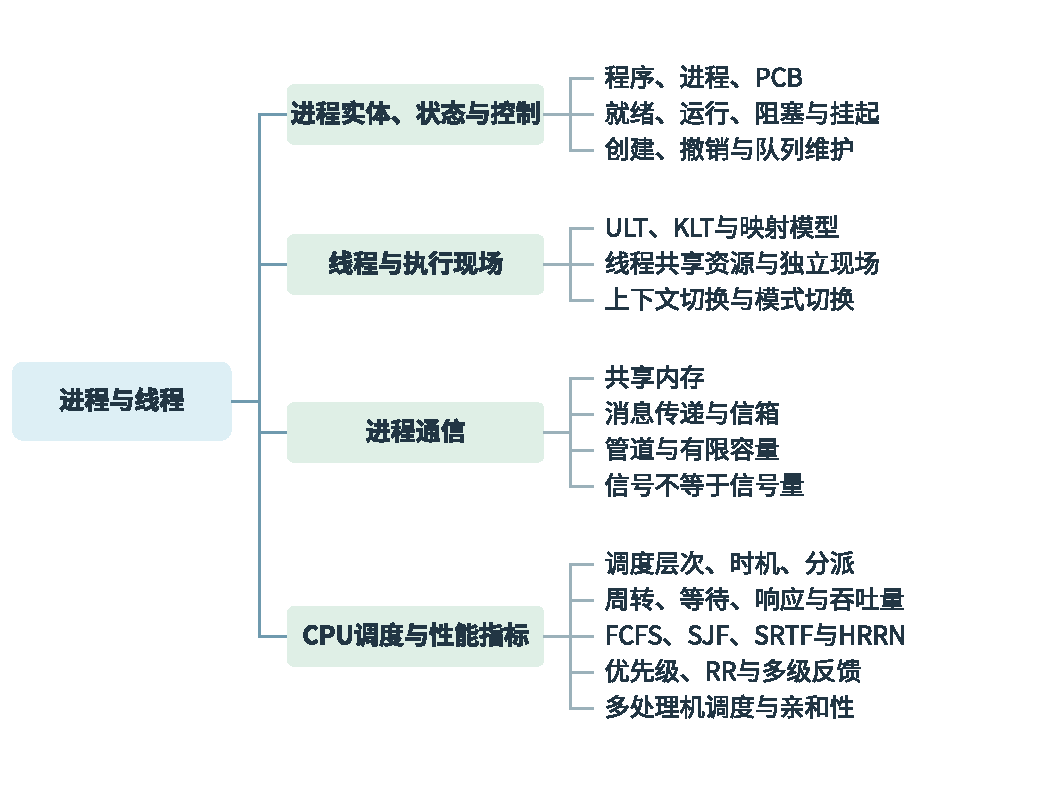
\includegraphics[width=\linewidth,height=168mm,keepaspectratio]{figures/map-01.pdf}\end{wideblock}\par\medskip\clearpage

\par\medskip\noindent\textbf{知识导图（续）}\par\smallskip
\begin{wideblock}\centering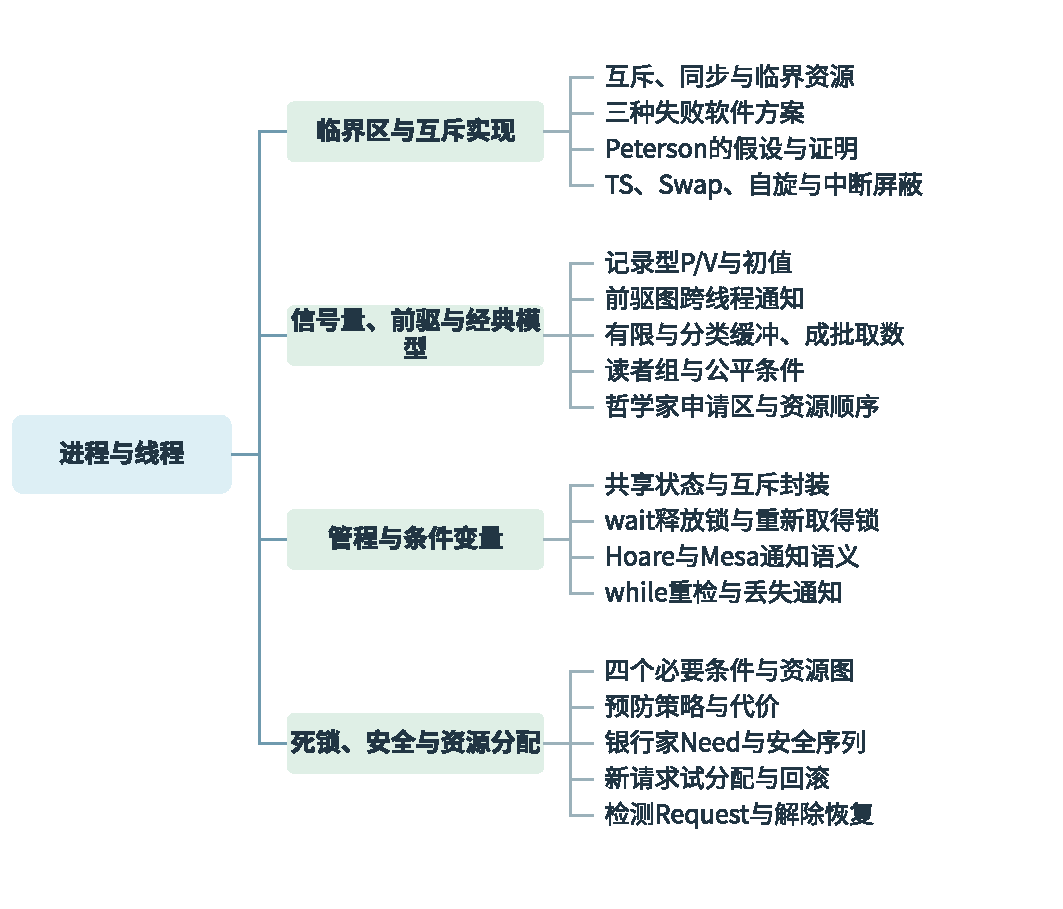
\includegraphics[width=\linewidth,height=168mm,keepaspectratio]{figures/map-02.pdf}\end{wideblock}\par\medskip\clearpage

\section{依导图建立``状态---时间---许可---资源''四本账}\label{OS02-guide}

\begin{methodbox}[先选模型，再做计算]

\begin{enumerate}
\def\labelenumi{\arabic{enumi}.}
\tightlist
\item
  进程题：列当前状态、所缺事件与所在队列，分开唤醒和分派。
\item
  调度题：列已到达候选集、剩余CPU时间、同刻事件次序与切换开销，沿时间线推进。
\item
  并发题：列共享状态、先决条件、许可初值、持锁区间，手推最空、最满与交错轨迹。
\item
  资源题：分清最大Need和当前Request，按资源种类逐项比较；试分配必须能回滚。
\end{enumerate}

\end{methodbox}

本章将进程与CPU调度、同步互斥、死锁三组知识放在同一教材章内。例题编号分别以2A、2B、2C区分三组，避免把调度时刻、信号量计数和资源向量混用。

\begin{definition}[把执行、协调和资源分配分开建模]

进程描述程序的一次执行及其资源环境；线程描述执行流。调度决定谁取得CPU，同步互斥决定哪些操作可先后或重叠，死锁分析判断已有资源等待能否解除。三者共用状态与队列，但需要不同的判据。

\end{definition}

\subsection{安全性检查的资源守恒推导}\label{OS02-conservation-proof}

\begin{theorem}[假定一个进程完成后的净资源变化]

若当前可用向量为Work，进程已持有Allocation，尚需Need，并且\(Need\le Work\)逐项成立，则假定它取得所需资源并有限完成后，新可用量为\(Work+Allocation\)。

\end{theorem}

\begin{proof}[借出和归还相抵]

先给足Need后，可用量暂为\(Work-Need\)；该进程完成时归还其全部持有量\(Allocation+Need\)。两项相加得\(Work-Need+Allocation+Need=Work+Allocation\)。逐项不等式保证借出前资源足够；有限完成与归还是假设条件。这个过程是安全性的假想证据，并非真的运行进程，也不能把当前不存在的资源加入Work。

\end{proof}

\section{进程、线程、调度与上下文切换}\label{OS02-module-02}

程序是指令和数据的静态描述，进程是程序的一次执行过程及其资源环境。同一可执行文件运行两次，可以产生两个进程；同一进程又可以包含多个执行线程。判断状态变化时，要分别问：资源属于谁，当前谁在执行，谁还在等一个事件，谁只是等待处理器。

\subsection{进程与线程：资源单位和执行单位}\label{OS02-2-1}

\textbf{进程}是系统进行资源分配和管理的基本单位，具有独立的运行状态和地址空间视图。进程实体通常由程序段、相关数据和进程控制块 PCB 等构成。PCB 记录标识、状态、调度信息、资源使用信息及保存的处理器现场，内核据此管理进程；``一个进程没有正在占用 CPU''不等于它不存在。

\textbf{线程}是进程内部的一条执行流。在引入线程的系统中，处理器调度通常落实到可调度线程，而地址空间、打开文件等资源主要归所属进程。每条线程需要自己的程序计数器、寄存器现场、栈和线程控制信息，否则无法分别记住执行位置和函数调用链。

同一进程的线程可以访问共同的代码、静态数据、堆及进程资源，但拥有独立的执行现场。``线程有自己的栈''指的是各线程的函数调用状态分别管理，但这不意味着同进程的其他线程在地址上无法访问该栈。只要得到有效地址并具备权限，线程仍可能错误地访问另一线程的对象；私有用途与硬件隔离不同。

进程通常具有动态性、并发性、独立性和异步性。独立性指其运行和管理环境，不表示不能通信或共享；异步性也不意味着可以违反自身指令的必要依赖。线程有利于把服务器中等待网络、处理请求等活动组织成多个执行流，但线程数增加同样会带来同步、栈空间和切换开销。

\begin{wideblock}

\par\medskip\noindent\begin{minipage}{\linewidth}\fontsize{9.3}{12}\selectfont\begin{tabularx}{\linewidth}{@{}YYY@{}}
\toprule\noalign{}
\begin{minipage}[b]{\linewidth}\raggedright
比较维度
\end{minipage} & \begin{minipage}[b]{\linewidth}\raggedright
不同进程之间
\end{minipage} & \begin{minipage}[b]{\linewidth}\raggedright
同一进程的不同线程之间
\end{minipage} \\
\midrule\noalign{}


资源与地址空间 & 各有地址空间和进程资源；共享须按机制建立 & 共享代码、数据、堆和打开文件等所属进程资源 \\
执行现场 & 由各自的控制信息保存 PC、寄存器、栈等 & 每条线程仍有独立 PC、寄存器、栈和线程控制信息 \\
切换要改变什么 & 还需切换相应地址空间环境 & 通常无需更换所属进程的地址空间，仍须换执行现场 \\
数据交换 & 通过共享内存、消息、管道等机制 & 可直接访问共同对象，仍须处理同步与互斥 \\
隔离边界 & 默认地址隔离有助限制误写的影响 & 一个线程可破坏共同空间；线程栈并非在地址上对其他线程不可访问 \\
\bottomrule\end{tabularx}
\end{minipage}\par\medskip

\end{wideblock}

这里比较的是资源归属；能否由内核分别调度、阻塞是否牵连其他线程，还要看下一节的线程实现与映射模型。

\subsection{就绪、运行和阻塞：先判断缺少什么}\label{OS02-2-2}

\textbf{就绪态}表示除处理器外，执行所需条件已满足；\textbf{运行态}表示正在处理器上执行；\textbf{阻塞态}表示等待 I/O、资源、同步事件等条件，暂不能因获得 CPU 就继续。单处理器同一时刻至多一个相应执行实体在运行，就绪与阻塞却都可以有多个。

\par\medskip\noindent\begin{minipage}{\linewidth}
\centering
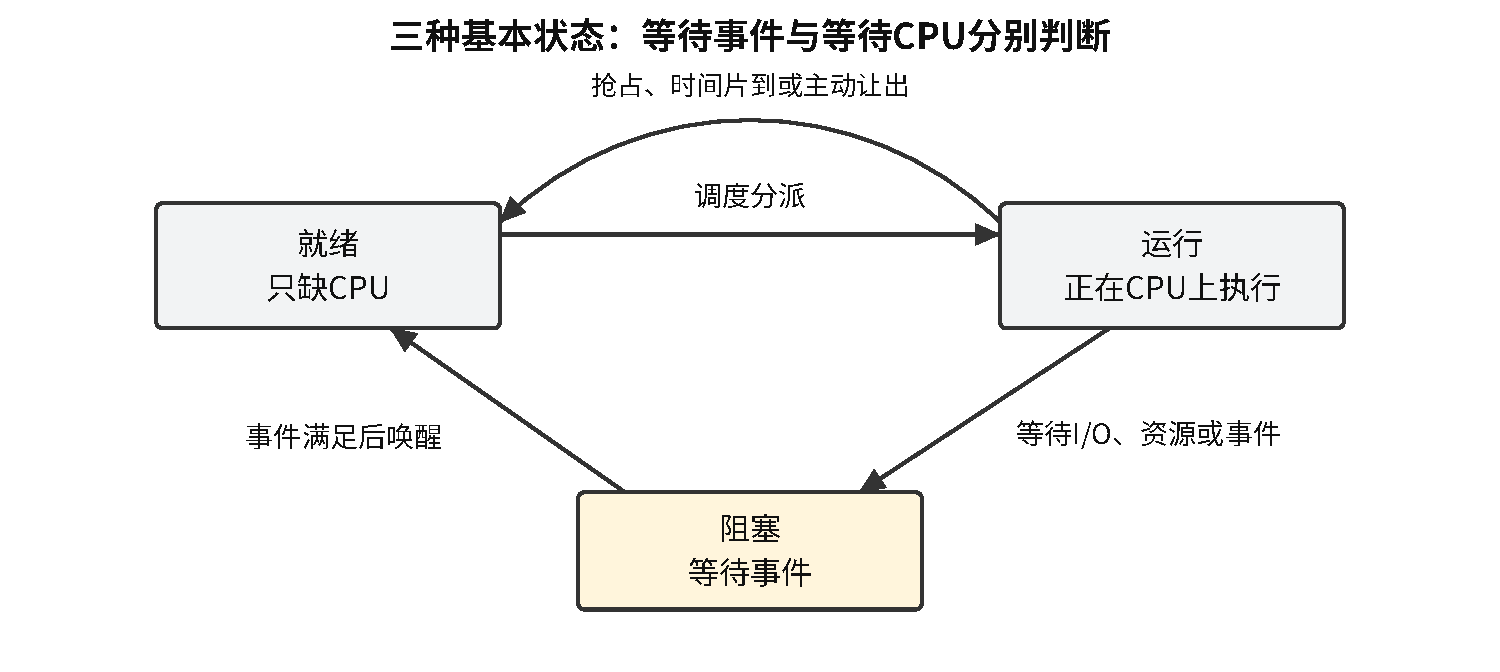
\includegraphics[width=\linewidth,height=125mm,keepaspectratio]{figures/OS_process_states.pdf}
\captionof{figure}{唤醒先进入就绪，调度以后才运行；箭头上的条件不能省略}\label{os-fig-states}
\end{minipage}\par\medskip

运行者用完时间片或被更高优先级者抢占，通常转为就绪；执行阻塞式 I/O 而数据未就绪，转为阻塞；等待事件发生后，由内核唤醒为就绪。阻塞者一般不能直接跳到运行，因为事件满足与分配处理器是两个决定。就绪者没有在执行，也不能主动发起一项新的阻塞操作。

创建态用于建立运行环境，终止态用于退出和清理；若进程被换出内存，还可引入挂起就绪、挂起阻塞等状态。挂起描述的是进程是否驻留内存，阻塞描述的是缺少事件，二者不是同义词。等待事件已满足的挂起阻塞进程，可以先成为挂起就绪，仍须调入并获得 CPU 才能运行。

\subsubsection{例 2A-1　主动让出处理器后去哪里}\label{OS02-ex2-1}

\begin{example}[配套例题]

【配套例题】 下列由当前线程引起的事件或执行的操作中，可能导致该线程由执行态变为就绪态的是（　）。

A. 键盘输入　　B. 缺页异常　　C. 主动出让 CPU　　D. 执行信号量的 wait() 操作

\end{example}

\textbf{解析。} 主动出让处理器时，线程可能仍具备执行条件，只是把本次运行机会交出去，因而变为就绪，答案为 \textbf{C}。缺页且需等待调页、等待未到来的输入，通常使线程阻塞。信号量 wait 若能取得许可，可继续运行；若取不到，则阻塞，而不是仅因调用了 wait 就进入就绪。

键盘输入或另一进程退出临界区，可能满足某个阻塞者等待的条件，使它被唤醒；当前进程的时间片用完则主要改变当前运行者的状态。判断``可能唤醒''时要指明被满足的是哪个等待条件，不能把所有调度事件都当作唤醒。

\subsection{用户级、内核级线程与映射模型}\label{OS02-2-3}

\textbf{用户级线程}由用户空间线程库建立和管理，内核可能只看见承载它们的进程或少量内核调度实体。纯用户级线程切换可以只修改用户现场，开销较小；但在多对一模型中，一个承载实体因阻塞式系统调用被阻塞，其他用户线程也失去在该实体上执行的机会；内核也无法把这些用户线程分派到多个核真正并行。

\textbf{内核级线程}由内核识别、管理和调度。某线程阻塞时，同进程的其他内核线程仍可运行；多个线程也可分派到不同核。代价是创建、管理和切换通常需要内核参与；因此``切换开销小''是用户级线程的长处，不能反过来算作内核级线程的优势。

\begin{wideblock}

\par\medskip\noindent\begin{minipage}{\linewidth}\fontsize{9.3}{12}\selectfont\begin{tabularx}{\linewidth}{@{}YYY@{}}
\toprule\noalign{}
\begin{minipage}[b]{\linewidth}\raggedright
共同维度
\end{minipage} & \begin{minipage}[b]{\linewidth}\raggedright
用户级线程 ULT
\end{minipage} & \begin{minipage}[b]{\linewidth}\raggedright
内核级线程 KLT
\end{minipage} \\
\midrule\noalign{}


谁维护线程控制信息 & 用户空间的线程库 & 操作系统内核 \\
谁选择这一级的运行者 & 线程库选择某个承载实体内的用户线程 & 内核调度器选择可运行的内核线程 \\
切换怎样发生 & 纯用户级切换可只保存、恢复用户现场，不必进入内核 & 由内核保存、恢复相应执行现场并分派 \\
内核能区分到哪一级 & 不能分别调度其不可见的用户线程，只能调度承载实体 & 可分别阻塞、唤醒和分派各内核线程 \\
\bottomrule\end{tabularx}
\end{minipage}\par\medskip

\end{wideblock}

是否牵连其他线程、能否多核并行，还要看这些管理对象在下表中如何映射，不能仅凭``用户级''三个字判断所有实现。

\begin{wideblock}

\par\medskip\noindent\begin{minipage}{\linewidth}\fontsize{9.3}{12}\selectfont\begin{tabularx}{\linewidth}{@{}YYY@{}}
\toprule\noalign{}
\begin{minipage}[b]{\linewidth}\raggedright
映射
\end{minipage} & \begin{minipage}[b]{\linewidth}\raggedright
内核看到什么
\end{minipage} & \begin{minipage}[b]{\linewidth}\raggedright
阻塞和并行的结果
\end{minipage} \\
\midrule\noalign{}


多对一 & 多个用户线程对应一个内核执行实体 & 一个阻塞可能挡住全部；不能在多核上同时执行这些用户线程 \\
一对一 & 每个用户线程对应一个内核线程 & 阻塞影响可局部化，可多核并行；内核管理成本较大 \\
多对多 & 多个用户线程复用若干内核线程 & 线程库与内核分层调度，并行度受可用内核线程和核数约束 \\
\bottomrule\end{tabularx}
\end{minipage}\par\medskip

\end{wideblock}

``内核级''描述管理方式，不能理解成该线程的应用代码始终在内核态执行。用户线程进入系统调用时也可能执行内核代码。线程类型、CPU 当前模式、进程所属地址空间是三个不同判断维度。

\subsection{创建、撤销与组织：PCB 为什么是管理入口}\label{OS02-2-4}

创建进程一般需要分配标识和 PCB、建立地址空间和初始数据、关联资源、初始化执行现场，再加入适当的调度队列。用户登录、启动程序或系统创建服务进程可能触发创建；给已有进程分配设备只是改变其资源状态，不必产生新进程。

终止进程时，内核停止其执行，处理相关等待与通知，回收资源并释放管理结构。子进程是否随父进程终止，取决于系统的父子关系政策；不能把级联终止当成所有系统的通则。某些系统会保留最少退出信息，供父进程取得状态后再完全释放。

PCB 可以用链表、队列或索引表组织。就绪队列按调度规则组织可运行者，事件等待队列组织等待同类条件者；状态转换时要同步维护状态字段和所在队列。不能只改一个``状态字''，却把进程留在错误的队列中。

线程的创建同样要建立 TCB、栈和初始执行现场，但可以复用所属进程的地址空间等资源。在常规父子进程模型中，父子是两个独立进程，可并发执行、有不同 PCB；即使最初采用写时复制暂时共享物理页，也不是共用一个无区分的虚拟地址空间。真正共享的部分须由共享映射等机制建立。

\subsection{共享内存、消息、管道和信号}\label{OS02-2-5}

\textbf{共享内存}让多个进程把某些虚拟地址映射到共同的物理存储区。建立映射后，数据交换可以通过普通访存完成，减少反复拷贝；但谁先写、读者何时可读、多个修改者是否冲突，仍需要同步机制。共享内存本身并不保证不发生竞争。

\textbf{消息传递}把数据交给消息接口，由发送、接收及相关队列组织通信。直接通信指定对方进程，间接通信通过信箱或端口；同步发送、异步发送等语义由接口规定。一次接收若没有消息，可能阻塞，也可能立即报告暂不可用，不能只凭``消息传递''决定状态。

\textbf{管道}提供有次序的数据流通道。经典无名管道常用于有亲缘关系的进程，通常按半双工模型理解；双向通信可用两个管道。命名管道允许按名称建立联系。管道容量有限，空管道上的阻塞读、满管道上的阻塞写都会等待；写入数据后，不代表读取者会立即得到 CPU。

\textbf{信号}是向进程通知某类事件的机制，如终止请求、定时事件等。信号与信号量不同：前者通知事件，后者通过许可计数和等待队列协调资源与次序。普通信号并不携带任意大量的数据，也不等同于可靠的消息队列；是否排队等细节须看具体信号类型与接口。

例如父进程经管道把一批数交给子进程：父进程先写数据，子进程读到数据后计算。管道本身组织数据和读写等待；若两者还要更新另一个共享统计量，就仍需为该统计量建立同步保护。不要把``已经用了一种通信方法''推成``所有共享状态都已受保护''。

\subsection{调度层次与评价指标}\label{OS02-2-6}

\textbf{高级调度}从后备作业中选作业进入内存并取得参与运行的资格；\textbf{中级调度}通过换出、换入调节内存中的进程数量；\textbf{低级调度}从就绪实体中选择处理器使用者。并非所有现代系统都以经典批处理作业队列组织这三级调度，但三者处理的对象和时间尺度应区分。

设作业或进程 \(i\) 的到达时刻为 \(A_i\)，首次运行时刻为 \(S_i\)，完成时刻为 \(C_i\)，实际服务时间为 \(B_i\)。在只含一个 CPU 段、无 I/O、忽略切换开销的题目中：

\[
T_i=C_i-A_i,\qquad W_i=T_i-B_i,\qquad R_i=S_i-A_i,\qquad T_i^{\mathrm{w}}=\frac{T_i}{B_i}.
\]

\(T_i\) 为周转时间，\(W_i\) 为就绪等待时间，\(R_i\) 为响应时间，\(T_i^{\mathrm{w}}\) 为带权周转时间。平均值是逐个算完再取算术平均；平均带权周转时间一般不等于平均周转时间除以平均运行时间。

若进程有 I/O 等待，周转时间还包含阻塞时间，此时不能只用 \(T_i-B_i\) 当作就绪等待；应再扣除相应阻塞时间。吞吐量是单位时间完成的任务数，CPU 利用率是观察区间内 CPU 忙时长占比。题目是否把切换时间计为``忙''，以及忙于内核开销是否算有效服务，需要按口径说明。

\subsection{什么时刻可以调度，抢占改变了哪一步}\label{OS02-2-7}

当前进程结束、主动阻塞或让出处理器，必须考虑选择其他可运行者；新进程到达、I/O 完成使更合适者就绪、时间片到期，也可能触发重新选择。\textbf{非抢占方式}允许当前运行者继续，直到结束或主动放弃；\textbf{抢占方式}允许在满足规则的事件点中断当前运行者，把它放回就绪队列。

调度器负责选择，分派器负责把处理器实际交给所选者，包括必要的现场恢复与切换。发生一次中断不必更换运行者，检查一次调度条件也不等于一定发生进程切换。题目询问``调度次数''时，应核清是否计首次分派、是否计选择原进程、是否计最后转入空闲；不能把事件点数和切换次数混算。

内核维护调度结构时，短小临界区等处不允许任意抢占，否则可能读到队列的半更新状态；处理中断的阶段也有相应约束。所谓内核可抢占，并非每条内核指令都可以无条件中断并调度。

\subsection{沿时间线执行调度算法}\label{OS02-2-8}

处理调度题时，先明确到达时间、服务时间、抢占规则、同刻事件次序及开销。每到一个可能改变选择的事件点，只在\textbf{已经到达且就绪}的进程中选择，记录剩余 CPU 时间。最后用完成时刻计算指标，并检查 CPU 总服务量是否与题表一致。

\subsubsection{FCFS、SJF、SRTF 与高响应比}\label{OS02-auto-1}

\textbf{先来先服务 FCFS}按就绪到达次序选择，通常不抢占。长 CPU 段在前时，后面的短进程和 I/O 型进程可能等很久，产生护航效应。\textbf{短作业/短进程优先 SJF}在选择时挑预计运行时间最短者，通常指非抢占版本；它需要预测运行时间，持续到来的短任务可能使长任务饥饿。

\textbf{最短剩余时间优先 SRTF}是抢占版本，新进程到达时比较的是``新进程的服务时间''与``当前进程剩余时间''，不能拿当前进程最初总时间比较。\textbf{高响应比优先 HRRN}通常非抢占，选择时计算

\[\text{响应比}=\frac{\text{等待时间}+\text{预计服务时间}}{\text{预计服务时间}}=1+\frac{W}{B}.\]

等待越久，响应比越大，有助于缓解长任务长期等候。这个``响应比''是调度优先量，与前节的``响应时间''不是同一个指标。

\subsubsection{例 2A-2　先排除尚未到达者，再比较}\label{OS02-ex2-2}

\begin{example}[配套例题]

【配套例题】 4 个作业到达系统的时刻和运行时间如下表所示。

\begin{wideblock}

\par\medskip\noindent\begin{minipage}{\linewidth}\fontsize{9.3}{12}\selectfont\begin{tabularx}{\linewidth}{@{}YYY@{}}
\toprule\noalign{}
作业 & 到达时刻 & 运行时间 \\
\midrule\noalign{}


J1 & 0 & 3 \\
J2 & 1 & 3 \\
J3 & 1 & 2 \\
J4 & 3 & 1 \\
\bottomrule\end{tabularx}
\end{minipage}\par\medskip

\end{wideblock}

系统在 \(t=2\) 时开始作业调度。若分别采用先来先服务和短作业优先调度算法，则选中的作业分别是（　）。

A. J2、J3　　B. J1、J4　　C. J2、J4　　D. J1、J3

\end{example}

\textbf{解析。} 此时只有 J1、J2、J3 到达。FCFS 选择最早到达的 J1；SJF 比较三者运行时间 3、3、2，选择 J3。答案为 \textbf{D}。J4 尚未到达，即使其时间最短也不能提前选择。

\textbf{原创变式。} 沿用本题数据，仅把算法改为 HRRN，检查它与 SJF 是否等同。\(t=2\) 时，J1、J2、J3 的响应比分别为 \(1+2/3\)、\(1+1/3\)、\(1+1/2\)，应选 J1。改变的是优先量，因此不能仍然只比较运行时长。

\subsubsection{优先级：先看数值方向，再看是否抢占}\label{OS02-auto-2}

优先级可以由任务性质静态规定，也可以随等待、CPU 使用等动态调整。数值大代表高还是低，必须按题目读；同为``优先级调度''不保证使用同一方向。提高长等候者优先级称为老化，有助于避免低优先级进程饥饿；实时任务则常需要按紧迫性或期限组织优先次序。

\subsubsection{例 2A-3　被抢占者的剩余时间必须保留}\label{OS02-ex2-3}

\begin{example}[配套例题]

【配套例题】 进程进入就绪队列的时刻、优先级（值越大优先权越高）及 CPU 执行时间如下表所示。

\begin{wideblock}

\par\medskip\noindent\begin{minipage}{\linewidth}\fontsize{9.3}{12}\selectfont\begin{tabularx}{\linewidth}{@{}YYYY@{}}
\toprule\noalign{}
进程 & 到达 & 优先级 & CPU 时间 \\
\midrule\noalign{}


P1 & 0 ms & 1 & 60 ms \\
P2 & 20 ms & 10 & 42 ms \\
P3 & 30 ms & 100 & 13 ms \\
\bottomrule\end{tabularx}
\end{minipage}\par\medskip

\end{wideblock}

采用基于优先权的抢占式 CPU 调度算法，从 0 ms 开始调度，三个进程的平均周转时间为（　）。

A. 60 ms　　B. 61 ms　　C. 70 ms　　D. 71 ms

\par\medskip\noindent\begin{minipage}{\linewidth}
\centering
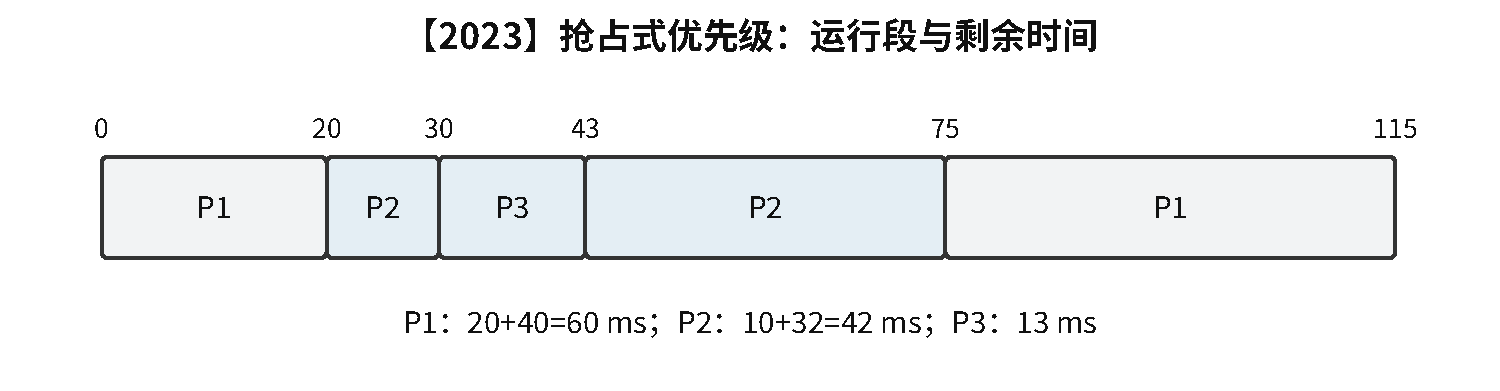
\includegraphics[width=\linewidth,height=125mm,keepaspectratio]{figures/OS_priority_timeline.pdf}
\captionof{figure}{每次抢占保留剩余时间，不重新开始整个 CPU 段}\label{os-fig-priority}
\end{minipage}\par\medskip

\end{example}

\textbf{解析。} 0---20 ms 只有 P1，执行 20 ms 后还余 40 ms。P2 到达并抢占，执行至 30 ms，还余 32 ms。P3 优先级最高，30---43 ms 执行完毕；随后 P2 执行 32 ms，于 75 ms 完成；最后 P1 执行 40 ms，于 115 ms 完成。

三者周转时间依次为 \(115-0=115\) ms、\(75-20=55\) ms、\(43-30=13\) ms，平均为 \((115+55+13)/3=61\) ms，答案为 \textbf{B}。完成时刻之和不是周转时间之和；每项都要减各自到达时刻。

\subsubsection{例 2A-4　一次到达不必增加一次进程调度}\label{OS02-ex2-4}

\begin{example}[配套例题]

【配套例题】 P0、P1、P2、P3 的到达、优先级（值越小优先权越高）和执行时间如下表所示。采用基于优先权的抢占式进程调度，从 0 ms 开始，到四个进程都运行结束为止，发生进程调度的总次数为（　）。

\begin{wideblock}

\par\medskip\noindent\begin{minipage}{\linewidth}\fontsize{9.3}{12}\selectfont\begin{tabularx}{\linewidth}{@{}YYYY@{}}
\toprule\noalign{}
进程 & 到达 & 优先级 & CPU 时间 \\
\midrule\noalign{}


P0 & 0 ms & 15 & 100 ms \\
P1 & 10 ms & 20 & 60 ms \\
P2 & 10 ms & 10 & 20 ms \\
P3 & 15 ms & 6 & 10 ms \\
\bottomrule\end{tabularx}
\end{minipage}\par\medskip

\end{wideblock}

A. 4　　B. 5　　C. 6　　D. 7

\end{example}

\textbf{解析。} 实际运行段依次为 P0{[}0,10)、P2{[}10,15)、P3{[}15,25)、P2{[}25,40)、P0{[}40,130)、P1{[}130,190)。P1 在 10 ms 到达，但优先级低于当时可选者，不单独取得一个运行段。按题目计首次分派且不计最后转入空闲，六次分派，答案为 \textbf{C}。若只数相邻两个实际运行进程的更换，则是五次；两种口径不可混用。

\subsubsection{时间片轮转与多级反馈队列}\label{OS02-auto-3}

\textbf{时间片轮转 RR}按就绪队列的先后，让每个进程取得至多一个时间片。进程在时间片内结束或阻塞，就提前让出；用完时间片仍未结束者回到队尾。时间片过长会接近 FCFS，过短会增加切换开销。若每次有效执行 \(q\)、切换耗时 \(s\)，持续满负荷时有效服务占比可近似写为 \(q/(q+s)\)，但最后一个短段等边界应逐段算。

同刻有新进程到达又有时间片到期时，谁先入队可能改变结果，应按题设；题设没有规定且确实影响答案时，必须声明采用的次序。不能把刚被抢占的进程总放在队首，新到者也不能越过当前时间片先运行。

\textbf{多级队列}把不同类型进程固定放在不同队列；\textbf{多级反馈队列}允许进程在队列间移动，常用较高队列的短时间片及时响应交互，CPU 使用时间较长者逐级下移。队列间是否抢占、各级规则和提升规则必须逐项读取，不能靠固定模板代替题设。

\subsubsection{例 2A-5　二级反馈中，第二级按剩余量选择}\label{OS02-ex2-5}

\begin{example}[配套例题]

【配套例题】 系统采用二级反馈队列调度。Q1 采用时间片轮转，时间片为 10 ms；Q2 采用短进程优先。系统优先调度 Q1，Q1 为空才调度 Q2；新创建进程先进入 Q1，在 Q1 执行一个时间片后仍未结束则转入 Q2。当前两队列为空，系统依次创建 P1、P2 后开始调度，两者需要的 CPU 时间分别为 30 ms、20 ms。平均等待时间为（　）。

A. 25 ms　　B. 20 ms　　C. 15 ms　　D. 10 ms

\end{example}

\textbf{解析。} P1 在 Q1 执行 0---10 ms，余 20；P2 执行 10---20 ms，余 10。此时 Q1 为空，Q2 中 P2 剩余较短，先执行 20---30 ms 完成，再运行 P1 至 50 ms。两者初始时均已创建，等待分别为 \(50-30=20\) ms、\(30-20=10\) ms，平均 15 ms，答案为 \textbf{C}。转入 Q2 以后，已经执行的时间不能重复计算。

\subsubsection{例 2A-6　同一组到达事件，SRTF 与 RR 如何分别推进}\label{OS02-ex2-6}

\begin{example}[配套例题]

〖2.2-006〗 系统有 4 个进程，预计运行时间和到达就绪队列的时刻如下，单位均为时间配额。分别采用可抢占式短进程优先和时间片轮转调度（时间片为 2），求各进程的调度次序与平均周转时间。

\begin{wideblock}

\par\medskip\noindent\begin{minipage}{\linewidth}\fontsize{9.3}{12}\selectfont\begin{tabularx}{\linewidth}{@{}YYY@{}}
\toprule\noalign{}
进程 & 到达时刻 & 预计运行时间 \\
\midrule\noalign{}


P1 & 0 & 8 \\
P2 & 1 & 4 \\
P3 & 2 & 9 \\
P4 & 3 & 5 \\
\bottomrule\end{tabularx}
\end{minipage}\par\medskip

\end{wideblock}

\end{example}

\textbf{解析。} SRTF 在 0 时先选 P1；到 1 时 P1 余 7，而 P2 只需 4，故抢占。到 2 时 P2 余 3，小于新来的 P3 的 9；到 3 时 P2 余 2，小于 P4 的 5，均不抢占。P2 在 5 完成后，等待者的剩余量依次为 P1 的 7、P3 的 9、P4 的 5，因此先 P4，再 P1，最后 P3。

\begin{wideblock}

\par\medskip\noindent\begin{minipage}{\linewidth}\fontsize{9.3}{12}\selectfont\begin{tabularx}{\linewidth}{@{}YYY@{}}
\toprule\noalign{}
进程 & SRTF 实际运行区间 & 周转时间 \\
\midrule\noalign{}


P1 & {[}0,1)、{[}10,17) & 17 \\
P2 & {[}1,5) & 4 \\
P3 & {[}17,26) & 24 \\
P4 & {[}5,10) & 7 \\
\bottomrule\end{tabularx}
\end{minipage}\par\medskip

\end{wideblock}

平均周转为 \((17+4+24+7)/4=13\)。P3、P4 到达都使调度器重新比较，但比较后可以继续当前 P2，不能把每次到达都强制切换。

RR 按本题参考解采用``同刻新到者先入队，再把时间片到期者放队尾''的约定。P1 在 {[}0,2) 后回队尾，此时队列为 P2、P3、P1；P4 在 3 到达，排在当时的等待队尾。以后按同样规则，每次只扣实际使用的一个时间片；剩余不足 2 者提前结束。

\begin{wideblock}

\par\medskip\noindent\begin{minipage}{\linewidth}\fontsize{9.3}{12}\selectfont\begin{tabularx}{\linewidth}{@{}YYY@{}}
\toprule\noalign{}
进程 & RR 实际运行区间 & 周转时间 \\
\midrule\noalign{}


P1 & {[}0,2)、{[}6,8)、{[}14,16)、{[}20,22) & 22 \\
P2 & {[}2,4)、{[}10,12) & 11 \\
P3 & {[}4,6)、{[}12,14)、{[}18,20)、{[}23,25)、{[}25,26) & 24 \\
P4 & {[}8,10)、{[}16,18)、{[}22,23) & 20 \\
\bottomrule\end{tabularx}
\end{minipage}\par\medskip

\end{wideblock}

平均周转为 \((22+11+24+20)/4=19.25\)。最后只有 P3，它在 25 用完一个片后仍可再次获选，不能因为``轮转''而强行等待一个不存在的其他进程。若同刻入队约定改变，2 时的队列及以后轨迹也要随之重算。

\subsubsection{调度算法的选择依据与抢占条件}\label{OS02-auto-4}

下表比较的是前述 CPU 调度规则。``需要时长''指选择时需要已知或估计的 CPU 服务量，不是说运行时间必须由用户准确预报。各种算法都只在已到达、已就绪的实体中选择。

\begin{wideblock}

\par\medskip\noindent\begin{minipage}{\linewidth}\fontsize{9.3}{12}\selectfont\begin{tabularx}{\linewidth}{@{}YYYY@{}}
\toprule\noalign{}
\begin{minipage}[b]{\linewidth}\raggedright
算法
\end{minipage} & \begin{minipage}[b]{\linewidth}\raggedright
下一个运行者怎样选
\end{minipage} & \begin{minipage}[b]{\linewidth}\raggedright
是否抢占
\end{minipage} & \begin{minipage}[b]{\linewidth}\raggedright
是否需要预计 CPU 时长
\end{minipage} \\
\midrule\noalign{}


FCFS & 按进入就绪队列的先后 & 通常不抢占 & 不需要 \\
SJF & 预计服务时间最短者 & 本章指非抢占版 & 需要预计服务时间 \\
SRTF & 预计剩余时间最短者 & 可以抢占 & 需要预计剩余时间 \\
HRRN & 选择 \(1+W/B\) 最大者 & 通常不抢占 & 需要预计服务时间 \(B\) \\
优先级 & 按题设优先级高低 & 两种版本都有 & 通常不以时长为必需输入 \\
RR & 队首运行至片满、结束或阻塞 & 片满时抢占 & 不需要 \\
多级反馈队列 & 先选队列，再执行该队列规则 & 常见模型允许高队列抢占 & 不需事先估计总服务时间 \\
\bottomrule\end{tabularx}
\end{minipage}\par\medskip

\end{wideblock}

\begin{wideblock}

\par\medskip\noindent\begin{minipage}{\linewidth}\fontsize{9.3}{12}\selectfont\begin{tabularx}{\linewidth}{@{}YY@{}}
\toprule\noalign{}
\begin{minipage}[b]{\linewidth}\raggedright
算法
\end{minipage} & \begin{minipage}[b]{\linewidth}\raggedright
等待方面的主要边界
\end{minipage} \\
\midrule\noalign{}


FCFS & 正常推进时不因后到者插队而饥饿；短任务可能被长任务拖住 \\
SJF & 持续到来的短任务可能使长任务饥饿 \\
SRTF & 比较剩余量；持续短任务同样可能阻挡长任务 \\
HRRN & 等待使响应比增加，兼顾长短任务；不等于固定等待上界 \\
优先级 & 固定低优先级者可能饥饿；老化可逐步提高其优先级 \\
RR & 同队列轮流获得机会；片过小会增加切换开销 \\
多级反馈队列 & 若高队列始终有任务，低队列可能长期无机会；是否定期提升须看规则 \\
\bottomrule\end{tabularx}
\end{minipage}\par\medskip

\end{wideblock}

``短任务优先''不自动包含抢占；``按优先级''也不自动包含时间片。题干同时给出多个规则时，先判断哪个规则决定候选队列，再判断队内顺序，最后处理到达、片满和阻塞等事件。

\subsubsection{例 2A-7　把``等待越久越优先''写成动态优先数}\label{OS02-ex2-7}

\begin{example}[配套例题]

【配套例题】 某进程调度程序采用基于优先数（priority）的调度策略，即选择优先数最小的进程运行。进程创建时由用户指定一个 nice 作为静态优先数。为了动态调整优先数，引入运行时间 cpuTime 和等待时间 waitTime，初值均为 0。进程处于执行态时，cpuTime 定时加 1，且 waitTime 置 0；进程处于就绪态时，cpuTime 置 0，waitTime 定时加 1。请回答下列问题。

（1）若调度程序只将 nice 的值作为进程的优先数，即 priority=nice，则可能会出现饥饿现象，为什么？

（2）使用 nice、cpuTime 和 waitTime 设计一种动态优先数计算方法，以避免产生饥饿现象，并说明 waitTime 的作用。

\end{example}

\textbf{解析。} （1）数值小才优先。若就绪队列中一直有 nice 较小的进程，nice 较大的进程便可能一直落选。系统仍有其他进程在运行，因此这是饥饿，不能解释成全部进程互等的死锁。

（2）一种方法是

\[priority=nice+k_1\,cpuTime-k_2\,waitTime,\qquad k_1>0,\ k_2>0.\]

运行时间增长使优先数增大，降低持续占用 CPU 者的优先级；就绪等待增长使优先数减小，提高长期等待者的优先级。两个符号都由``数值越小越优先''决定，不能沿用数值越大越优先的公式。

例如仅为检验公式方向，取 \(k_1=k_2=1\)：nice=10 的等待者在等待 11 个计时单位后，优先数成为 \ensuremath{-}1，比 nice=0 的刚就绪进程更小，因而先被选中。这是\textbf{原创代入检查}，不是原题新增数据。等待者一旦运行，waitTime 按题设清零；再次就绪时 cpuTime 清零，不能把这两个量误当成从创建起永久累计的总量。

waitTime 提供的是老化机制。但若把它用作无饥饿的保证，还需满足一些前提：采用通常的有限进程或有界 nice 模型，持续计时和重算，适当抢占或有限运行段，以及同优先数下不无限越过等待者。不能把一个公式解释成对任意到达流和任意调度实现都存在固定等待上界。

\subsection{多处理机调度：负载与缓存都有代价}\label{OS02-2-9}

多个处理器可以使用公共就绪队列，也可以各自维护队列。公共队列便于共享负载，但并发访问需同步；每核队列降低争用，却可能出现一核排队、一核空闲，需要负载均衡。推迁移由繁忙的处理器把任务移出，拉迁移由空闲的处理器取得任务。

\textbf{处理器亲和性}倾向让线程继续在此前运行的处理器上执行，利用缓存和地址转换缓存中的内容。软亲和性是调度倾向，硬亲和性是允许处理器集合的明确限制。负载均衡可能要求迁移，缓存局部性可能要求保留，二者需要权衡；不能把``每核进程数相同''当作负载完全相同，因为各任务剩余计算量可能不同。

同时多线程 SMT 让一个物理核维护多个硬件线程现场，共享某些执行资源；它不等于每条逻辑处理器都具有独立完整的执行单元。调度题未给多处理机规则时，不要自行把一个进程拆到多个核同时加速。

\subsection{上下文切换与模式切换}\label{OS02-2-10}

\textbf{上下文}是恢复执行所需的状态，包括程序计数器、寄存器、栈等；进程切换还可能更换地址空间相关状态。\textbf{模式切换}只是当前执行权限模式改变，例如同一进程进入系统调用再返回；它不必改变执行身份。\textbf{上下文切换}则把 CPU 从一个执行实体交给另一个。

同进程的线程切换通常要换 PC、寄存器和栈，而不必更换进程页表基址和共同的文件资源。跨进程切换还要建立新地址空间环境；TLB 是否必须全部清空，取决于是否支持地址空间标识等硬件条件。不能把``跨进程切换一定清空全部 Cache''列作一般步骤。

〖2.2-009〗 同一进程中 T1 切到 T2，需要更新各自执行位置和栈环境；进程页表和进程打开文件资源并不因同进程线程切换而自然改变。判断题列出的每项寄存器，要先说明它保存线程状态还是进程共享状态。

【配套例题】 ``执行系统调用''完成并返回调用者时，可以使 CPU 从内核态回到用户态；阻塞、唤醒和执行 CPU 调度本身属于内核管理路径，不能认为这些操作完成时都必然返回用户态。具体返回到哪个线程，由当时调度与返回路径决定。

\subsection{分支自测：用相同时间线检查不同问题}\label{OS02-2-review}

以下为原创回顾设问。

\begin{enumerate}
\def\labelenumi{\arabic{enumi}.}
\tightlist
\item
  已等到 I/O 数据的进程是否立即运行？线程发出 I/O 请求是否必然阻塞？
\item
  在例 2A-3中，P2 的响应时间、等待时间、周转时间分别是多少？
\item
  同一进程的两个内核线程切换，是否必须改页表基址？
\item
  预计服务时间相同的两个作业，HRRN 如何反映等待差别？
\item
  多核上迁移线程，一定能提高性能吗？
\end{enumerate}

\subsubsection{自测答案}\label{OS02-auto-5}

\begin{enumerate}
\def\labelenumi{\arabic{enumi}.}
\tightlist
\item
  数据到达使相应等待条件满足，通常先就绪，再等调度。若请求非阻塞或数据已可用，I/O 接口可不使线程阻塞。
\item
  P2 在到达 20 ms 时立即开始，响应时间 0；周转时间 55 ms，服务 42 ms，所以等待 13 ms。
\item
  通常不必，二者使用同一进程地址空间，但 PC、寄存器和线程栈等要切换。
\item
  \(B\) 相同则 \(1+W/B\) 随 \(W\) 增大，等待较久者响应比更高。
\item
  不一定。迁移可能缓解排队，也可能丢失缓存局部性、产生同步和迁移成本。
\end{enumerate}

\section{同步、互斥与信号量}\label{OS02-module-03}

进程合作时，需要回答两个不同的问题：一项操作必须等哪项操作完成，几个进程能否同时操作同一份共享数据。前者决定先后次序，后者决定互斥范围。信号量可以表达这两种约束，但其含义、初值和放置位置都要从题目条件推出。

本章代码是描述并发关系的伪代码。\texttt{P(\allowbreak{}S)\allowbreak{}} 与 \texttt{wait(\allowbreak{}S)\allowbreak{}} 同义，\texttt{V(\allowbreak{}S)\allowbreak{}} 与 \texttt{signal(\allowbreak{}S)\allowbreak{}} 同义；条件变量的 \texttt{wait}、\texttt{signal} 会另行定义。进程编号与数组下标从 0 开始。除特别说明外，信号量采用本章的记录型语义，不假定等待队列按先进先出调度。

\subsection{临界区约束什么，为什么还需要同步}\label{OS02-concepts}

\subsubsection{从一次丢失的更新看原子操作}\label{OS02-auto-6}

两个进程共享整数 \texttt{x}，初值为 0，各执行一次 \texttt{x=\allowbreak{}x+\allowbreak{}1}。一条高级语言语句未必对应一条不可分割的机器操作。若每次更新分为``读入本地寄存器---加 1---写回''，就可能出现下图的交错：两个进程都读到 0，最后都写入 1，结果只有 1。

\par\medskip\noindent\begin{minipage}{\linewidth}
\centering
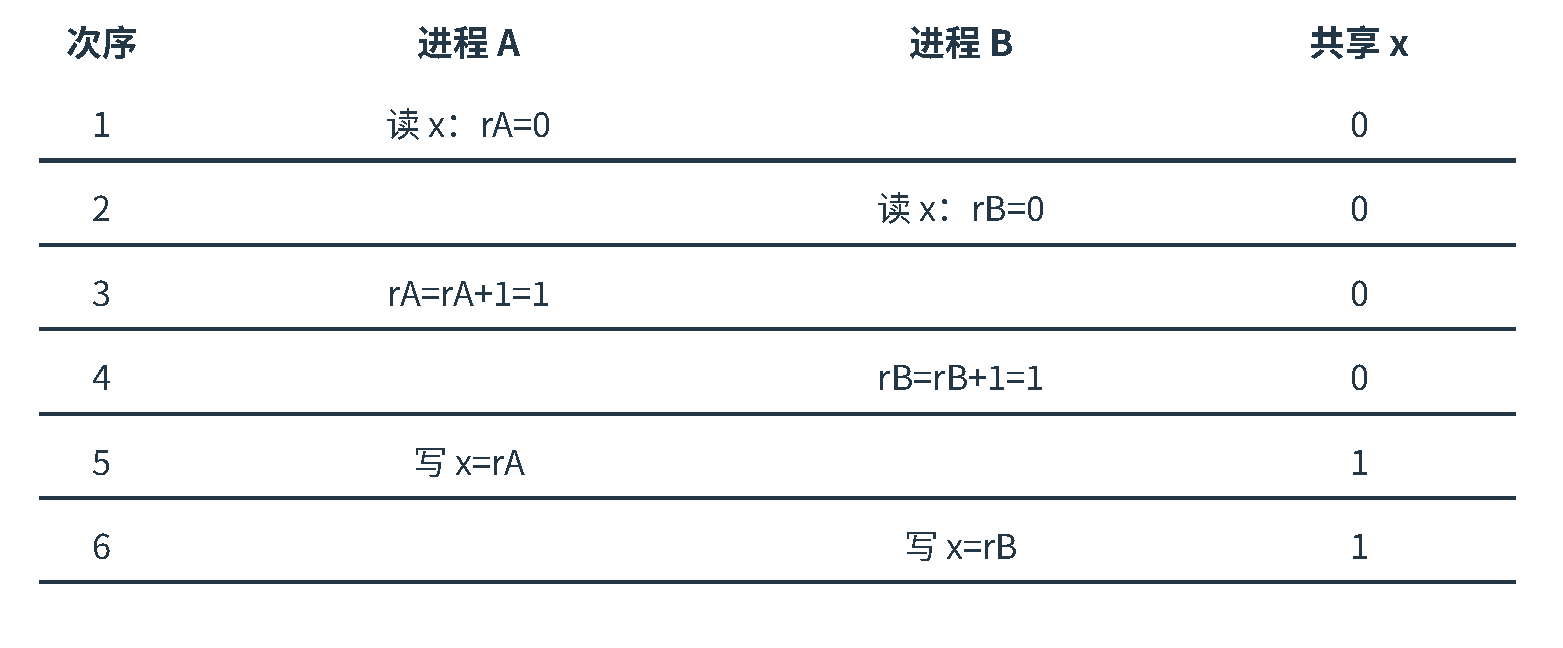
\includegraphics[width=\linewidth,height=125mm,keepaspectratio]{figures/F01_lost_update.pdf}
\captionof{figure}{两次更新都完成，但后一次写回覆盖了前一次结果}\label{fig-lost}
\end{minipage}\par\medskip

即使只有一个 CPU，进程也可能在读与写之间被切换出去，所以单处理机上同样存在竞争。多处理机上还可能真正同时执行。这里把某段操作视为\textbf{原子操作}，是说其他并发操作无法插入其内部，也无法观察到破坏该操作语义的中间状态；不能仅凭``这是一行代码''认定原子性。

进程在运行态时占用处理机；在就绪态时具备运行条件，等待调度；在阻塞态时等待事件，暂时不能被调度执行。因资源不足而主动阻塞，与反复执行检查指令的忙等待不同。唤醒把阻塞进程变为就绪进程，不保证它立即运行。

\subsubsection{资源、代码与先后关系}\label{OS02-auto-7}

\textbf{临界资源}是在同一时段只允许一个进程使用的共享资源。\textbf{临界区}是进程中访问相应临界资源的代码段。进入区负责申请进入，退出区负责释放；二者不属于被保护的临界区本身。资源是一份共享对象，相关临界区可以有多段，分布在不同进程中。

〖2.3-027〗 5 个并发进程各有一段访问同一变量 A 的代码，对应 5 个相关临界区。临界区要按代码段计数，不能按共享变量的份数计数。一般程序若在多处访问共享数据，也不能仅凭进程数推出代码段总数。

\textbf{互斥}限制重叠：某进程正在访问临界资源时，其他需要访问它的进程须等待。\textbf{同步}规定合作中的先后关系：后续操作需要某项结果，就必须等产生该结果的操作完成。同一对进程可能同时受这两种约束。

\subsubsection{例 2B-1　共享缓冲区中的两种约束}\label{OS02-ex-err11}

\begin{example}[配套例题]

〖2.3-011〗 进程 A 和进程 B 通过共享缓冲区协作完成数据处理，进程 A 负责产生数据并放入缓冲区，进程 B 从缓冲区读数据并输出。进程 A 和进程 B 之间的制约关系是（　）。

A. 互斥关系　　B. 同步关系　　C. 互斥和同步关系　　D. 无制约关系

\end{example}

\textbf{解析。} 进程 B 必须在进程 A 放入数据后读取，这是同步；对共享缓冲区的访问还须协调，避免操作冲突，这是互斥。答案为 \textbf{C}。选项 B 只概括了先后关系，没有涵盖互斥。

本题指出两类约束，并不意味着任何实现都必须恰好使用``一个同步量加一个互斥量''。操作是否反复执行、容量是否为 1，以及同步本身是否已排除重叠，都会影响实现；\hyperref[OS02-ex-2024]{例 2B-4}会分别处理。

\subsubsection{怎样判断互斥方案是否合格}\label{OS02-auto-8}

检查一种方案时，先找违反条件的具体交错，不要只看顺序执行的结果。

\begin{wideblock}

\par\medskip\noindent\begin{minipage}{\linewidth}\fontsize{9.3}{12}\selectfont\begin{tabularx}{\linewidth}{@{}YY@{}}
\toprule\noalign{}
\begin{minipage}[b]{\linewidth}\raggedright
检查项
\end{minipage} & \begin{minipage}[b]{\linewidth}\raggedright
要问的问题
\end{minipage} \\
\midrule\noalign{}


空闲让进 & 临界区无人使用，是否仍被一个不参与竞争的进程挡住？ \\
忙则等待 & 一个进程尚未退出，另一个能否进入同一临界区？ \\
有限等待 & 请求提出后，其他进程获准进入的次数是否存在有限上界？还须满足进程持续获得执行机会、临界区操作有限等前提。 \\
让权等待 & 不能进入时，是阻塞并让出处理机，还是继续占用 CPU 检查？ \\
\bottomrule\end{tabularx}
\end{minipage}\par\medskip

\end{wideblock}

前三项分别检查进入机会、互斥安全和等待上界；让权等待检查等待方式。一个自旋方案可能保证互斥，却不满足让权等待。\textbf{无死锁不等于无饥饿}：系统整体仍在前进，但某个进程可能反复被越过。

\subsection{软件互斥与锁：检查和占用必须连起来}\label{OS02-locks}

\subsubsection{三种失败方案留下了什么问题}\label{OS02-auto-9}

以下双进程模型假定单次共享变量读写原子、内存顺序与伪代码一致。\texttt{flag[i]} 表示进程 \(P_i\) 想进入。现代机器上的编译器重排与存储重排不在这些伪代码的默认模型内，实际程序还需相应原子变量与内存序保证。

\begin{wideblock}

\par\medskip\noindent\begin{minipage}{\linewidth}\fontsize{9.3}{12}\selectfont\begin{tabularx}{\linewidth}{@{}YYY@{}}
\toprule\noalign{}
\begin{minipage}[b]{\linewidth}\raggedright
方案
\end{minipage} & \begin{minipage}[b]{\linewidth}\raggedright
进入区的核心操作
\end{minipage} & \begin{minipage}[b]{\linewidth}\raggedright
一条足以否定它的执行情况
\end{minipage} \\
\midrule\noalign{}


单标志法 & 等待 \texttt{turn=\allowbreak{}=\allowbreak{}i}，退出时将机会交给对方 & \texttt{turn=\allowbreak{}0}，但 \(P_0\) 一直在剩余区工作（不访问该临界资源的其他代码）；\(P_1\) 不能进入空闲临界区。 \\
双标志先检查 & 先等对方 \texttt{flag} 为假，再置自己为真 & 双方都在对方置真前完成检查，随后同时进入，不能保证互斥。 \\
双标志后检查 & 先置自己为真，再等对方为假 & 双方先置真，都等待对方退出；此时没有任何一方进入，无法执行清标志。 \\
\bottomrule\end{tabularx}
\end{minipage}\par\medskip

\end{wideblock}

这些模型与反例见王道书 §2.3。先检查法的问题是``检查与声明占用分离''；简单调换两句又可能造成双方互等。

\subsubsection{Peterson 算法怎样处理双方同时申请}\label{OS02-auto-10}

Peterson 算法用 \texttt{flag} 表达意愿，用 \texttt{turn} 在双方都想进入时决定谁先进入。两个 \texttt{flag} 初值均为 \texttt{false}；对 \(i\in\{0,1\}\)，令 \(j=1-i\)：

\BlueLines{3}
\begin{codeblock}[language={}]
flag[i] = true;
turn = j;
while (flag[j] && turn == j) { }  // 忙等待
访问临界资源;
flag[i] = false;
\end{codeblock}

若只有自己请求，对方的 \texttt{flag} 为假，可直接进入。若双方都请求，两次对 \texttt{turn} 的写入总有先后：后写的一方把进入机会让给对方，自己等待。退出时清除自己的意愿，等待者随后通过检查。

还须排除``一个已进入，另一个又进来''的情况。假设 \(P_i\) 在临界区，此时 \texttt{flag[i]} 为真；后来的 \(P_j\) 声明意愿并将 \texttt{turn} 置为 \texttt{i}，就必须等待。如果双方已在进入区竞争，后一次 \texttt{turn} 写入同样使其中一方等候。由此排除同时进入。在上述内存模型、进程继续执行且临界区有限等前提下，它也能保证有限等待；它仍在循环检查，不能让权等待。

\subsubsection{TestAndSet 为什么能够上锁}\label{OS02-auto-11}

硬件提供的 TestAndSet（TS，也称 TSL）以一次原子操作返回 \texttt{lock} 的旧值，并把 \texttt{lock} 置为真。以下只是该指令的逻辑含义，不能把普通语言实现的三句代码直接当作原子指令：

\BlueLines{4,7}
\begin{codeblock}[language={}]
TestAndSet(lock):
    old = lock
    lock = true
    return old

// lock 初值 false
while (TestAndSet(lock)) { }
访问临界资源;
lock = false;
\end{codeblock}

第一个读到假值的调用者同时把锁置真；后续调用者得到真值，继续等待。关键在于``取旧值并置真''不能被其他竞争者插入，而不在于 \texttt{while} 语句本身有什么特殊之处。Swap/XCHG 则原子交换共享的 \texttt{lock} 与进程私有的 \texttt{key}。共享 \texttt{lock} 初值为假，每次申请先令本进程的 \texttt{key=\allowbreak{}true}，再反复原子交换二者，直到 \texttt{key=\allowbreak{}false}，表示取得了交换前的空闲锁；退出时令 \texttt{lock=\allowbreak{}false}。

这类锁若一直循环，就是\textbf{自旋锁}。它避免睡眠和唤醒的切换开销，适用于持锁时间很短、持锁者能够继续运行的情形。它不保证公平；有限等待也不能只从指令的原子性推出。阻塞锁在不可用时使线程睡眠，更适合可能较长的等待；不能把``互斥锁''这个名称一概等同于自旋实现。

单处理机上，自旋者正在运行时，持锁者不能同时运行；若调度还能让持锁者重新运行，锁仍可能被释放。若相关内核区又禁止了能让持锁者运行的切换，便不能指望忙等自行结束。多处理机上，其他核可继续执行持锁者。

屏蔽本 CPU 的可屏蔽中断，只能在单处理机、相关执行路径不会主动阻塞等限定下保护短小的内核临界操作；它无法阻止另一 CPU 访问共享数据，因此不适用于一般多处理机互斥。开关中断是特权操作，普通用户程序无权执行。分析原语的原子性时，应说明保护范围，不能笼统写``所有原语都靠关中断''。

\subsection{信号量：先说明它代表什么，再计算初值}\label{OS02-semaphore}

\subsubsection{记录型 P、V 的完整语义}\label{OS02-auto-12}

记录型信号量 \(S\) 包含整数 \texttt{value} 与等待队列。初始化只做一次；以后通过 P、V 改变状态。以下``修改计数---判断---入队或唤醒''须由系统实现为一个原子操作；但进程阻塞之后，整个等待期间并不因此变成不可调度的原子区。

\BlueLines{1,3,7}
\begin{codeblock}[language={}]
P(S):
    S.value = S.value - 1
    if S.value < 0:
        将当前进程加入 S 的等待队列并阻塞
        // 被唤醒后，本次 P 返回；不再次减 1

V(S):
    S.value = S.value + 1
    if S.value <= 0:
        从 S 的等待队列移出一个进程，将其置为就绪
\end{codeblock}

P 表示申请一个许可。减 1 后为 0，说明最后一个可用许可刚被取得，\textbf{此时不阻塞}；减 1 后小于 0，才说明本次申请需要等待。V 增加一个许可；加 1 后仍小于或等于 0，说明原先有人等待，需要把这个机会交给一个等待者。V 本身不会因资源不足而阻塞。

\texttt{value>\allowbreak{}0} 表示尚未分配的许可数；\texttt{value=\allowbreak{}0} 表示没有未分配许可，也没有在该量上等待的进程；\texttt{value<\allowbreak{}0} 时，\(-\mathrm{value}\) 是等待队列长度。这些解释采用上述记录型定义。整型信号量的另一种实现是在 \texttt{S<\allowbreak{}=\allowbreak{}0} 时循环检查，再取得许可；其计数通常不为负，且可能忙等，不能混用两套数值规则。

设两台同类打印机对应初值 2，A、B、C、D 先后申请，再由 A、B 归还；下图为便于追踪，假定按入队顺序唤醒。

\par\medskip\noindent\begin{minipage}{\linewidth}
\centering
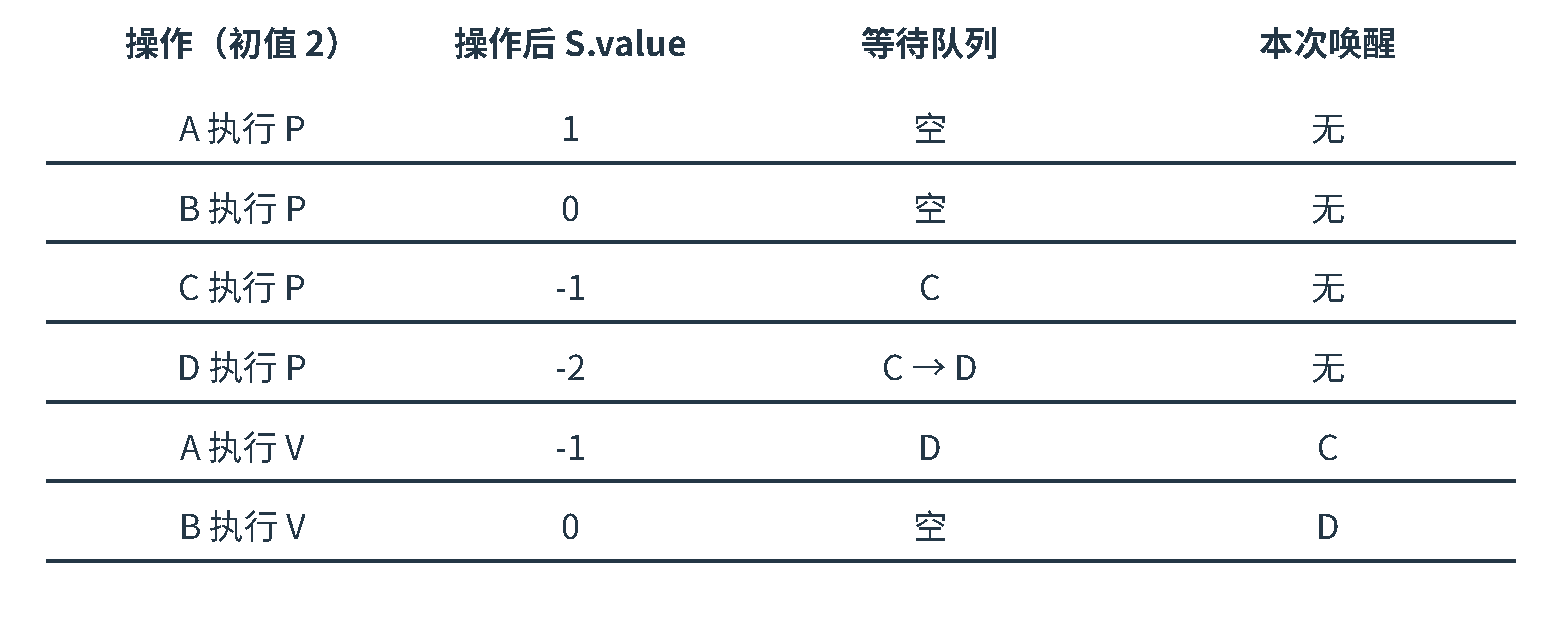
\includegraphics[width=\linewidth,height=125mm,keepaspectratio]{figures/F02_signed_semaphore.pdf}
\captionof{figure}{资源归还会唤醒一个等待者，计数不必先变为正数}\label{fig-signed}
\end{minipage}\par\medskip

A 归还后值为 \ensuremath{-}1，C 已得到可继续执行本次 P 的机会，D 仍等待。此时值仍为负数，但 C 不必再做一次 P。唤醒 C 也不意味着 C 立即运行：取得许可与分到 CPU 是两件事。

\subsubsection{初值来自初态，不来自``同步量''这个名称}\label{OS02-auto-13}

互斥量 \texttt{mutex=\allowbreak{}1} 表示只有一个进入许可。若某项一次性工作尚未完成，完成通知 \texttt{done=\allowbreak{}0}，后续进程先等通知。若缓冲区已有 \(k\) 个可消费的产品，产品许可应从 \(k\) 开始；容量为 \(n\)、已有 \(k\) 件时，空位许可应为 \(n-k\)。

\subsubsection{例 2B-2　同步信号量一定从 0 开始吗}\label{OS02-ex-err18}

\begin{example}[配套例题]

〖2.3-018〗 用 P、V 操作实现进程同步，信号量的初值为（　）。

A. \ensuremath{-}1　　B. 0　　C. 1　　D. 由用户确定

\end{example}

答案为 \textbf{D}。这里的``由用户确定''指根据资源或事件的初始状态确定，不能任意设数。B 适用于尚未发生、尚无可用结果的一次通知，不能覆盖所有同步情形。判断初值时，应检查题目有没有给出``尚未发生''这个限定。

\subsubsection{将完成条件放在正确位置}\label{OS02-auto-14}

若操作 B 必须在 A 完成后开始，设置 \texttt{done=\allowbreak{}0}：

\BlueLines{1,2}
\begin{codeblock}[language={}]
前进程：A; V(done);
后进程：P(done); B;
\end{codeblock}

若后进程先到，P 使它等待；若前进程先到，V 留下一个许可，后进程后来做 P 时也能通过。通知必须放在 A \textbf{完成之后}，不能在 A 开始前发布。互斥则是各参与者在受保护代码前 P、后 V；同步的一次 P 与产生它的一次 V 通常分布在不同进程中。因此，``P、V 要配合''不等于``必须在同一进程紧挨着出现''。

信号量通常没有互斥锁的持有者限制：一个进程可 P，另一个可 V。这允许它表达合作事件，也意味着不能把信号量与具有所有权要求的 mutex API 完全混同。

\subsection{从前驱图到线程代码}\label{OS02-precedence}

前驱图的边 \(A\to B\) 表示 B 不能在 A 完成前开始。先标出哪些顺序已由同一线程的程序顺序保证，再为剩下的跨线程依赖传递完成通知。给每条边各设一个初值 0 的信号量是常见的直接构造，但已有顺序可能使部分量不再需要；反过来，两个操作都等 C，也推不出它们之间要互相等待。

\subsubsection{例 2B-3　哪些边需要跨线程通知}\label{OS02-ex-2022}

\begin{example}[配套例题]

【配套例题】 某进程的两个线程 T1 和 T2 并发执行 A、B、C、D、E 和 F 共 6 个操作，其中 T1 执行 A、E 和 F，T2 执行 B、C 和 D。题46图表示上述 6 个操作的执行顺序所必须满足的约束：C 在 A 和 B 完成后执行，D 和 E 在 C 完成后执行，F 在 E 完成后执行。请使用信号量的 wait()、signal() 操作描述 T1 和 T2 之间的同步关系，并说明所用信号量的作用及其初值。

\par\medskip\noindent\begin{minipage}{\linewidth}
\centering
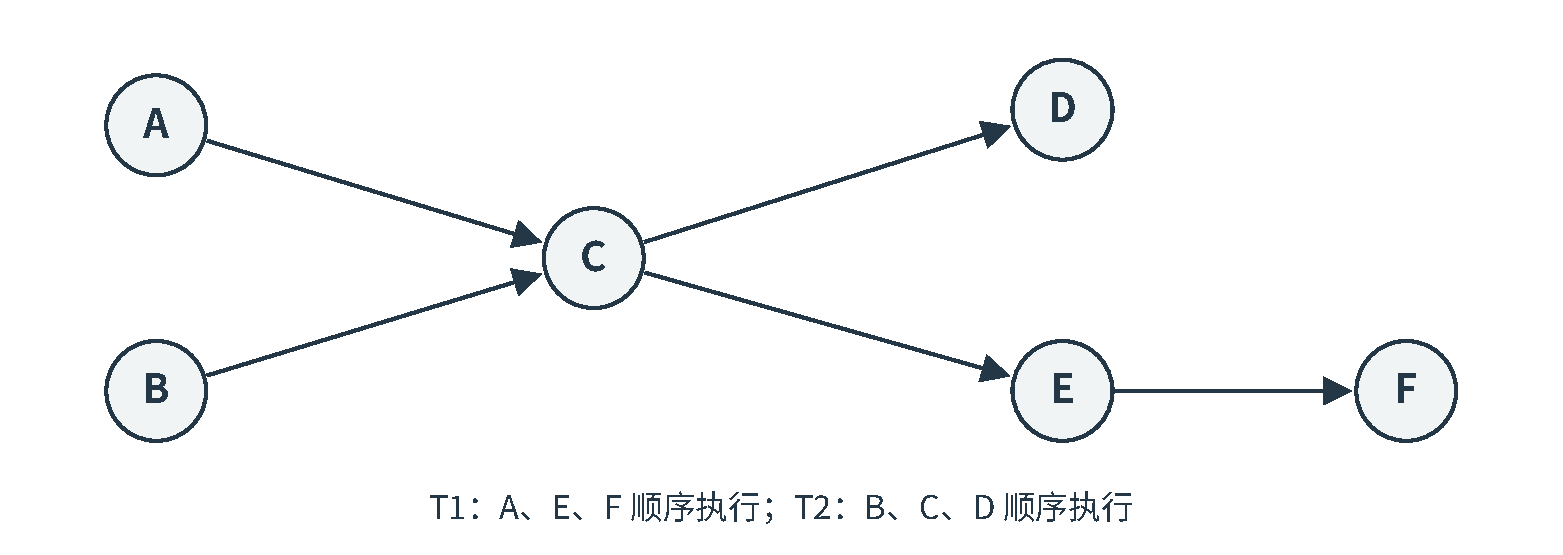
\includegraphics[width=\linewidth,height=125mm,keepaspectratio]{figures/F03_precedence_2022.pdf}
\captionof{figure}{原题前驱图；图下文字标明题干给出的线程归属}\label{fig-precedence}
\end{minipage}\par\medskip

\end{example}

\textbf{解析。} 在所写程序中，让 T1 按 A、E、F，T2 按 B、C、D 顺序执行，B\ensuremath{\to}C、C\ensuremath{\to}D、E\ensuremath{\to}F 就已满足。跨线程仍需保证 A\ensuremath{\to}C 和 C\ensuremath{\to}E，分别设 \texttt{S\_AC=\allowbreak{}0}、\texttt{S\_CE=\allowbreak{}0}。

\begin{codeblock}[language={}]
semaphore S_AC = 0, S_CE = 0;

T1() {                 T2() {
    A;                     B;
    signal(S_AC);          wait(S_AC);
    wait(S_CE);            C;
    E;                     signal(S_CE);
    F;                     D;
}                      }
\end{codeblock}

T2 到达 C 前已完成本线程的 B，又收到了 A 完成的通知，因此 C 的两个前提齐备。C 完成后先发布 \texttt{S\_CE}，T1 才能开始 E，随后执行 F；T2 自行继续 D。

例如，A、B、C、E、F、D 是允许的完成次序，A、B、C、D、E、F 也允许。D 与 E、F 没有额外次序要求。若把通知放到 D 后，虽然仍不违反图中的先后约束，却会强加 E 等待 D 的限制，减少题目允许的并发。结果安全不等于完整保留了题目允许的并发。

\subsection{缓冲区：容量许可与互斥范围分别建立}\label{OS02-buffer}

\subsubsection{例 2B-4　同一个缓冲区为什么有不同的信号量方案}\label{OS02-ex-2024}

\begin{example}[配套例题]

【配套例题】 计算机系统中的进程之间往往需要相互协作以完成一个任务。在某网络系统中，缓冲区 B 用于存放一个数据分组，对 B 的操作有 C1、C2 和 C3。C1 将一个数据分组写入 B 中，C2 从 B 中读出一个数据分组，C3 对 B 中的数据分组进行修改。要求 B 为空时才能执行 C1，B 非空时才能执行 C2 和 C3。

（1）假设进程 P1 和 P2 均需要执行 C1，实现 C1 的代码是否为临界区？为什么？（2分）

（2）假设 B 初始为空，进程 P1 执行 C1 一次，进程 P2 执行 C2 一次。请定义尽可能少的信号量，并用 wait()、signal() 操作描述进程 P1 和 P2 之间的同步或互斥关系，说明所用信号量的作用及其初值。（3分）

（3）假设 B 初始不为空，进程 P1 和 P2 各执行 C3 一次。请定义尽可能少的信号量，并用 wait()、signal() 操作描述进程 P1 和 P2 之间的同步或互斥关系，说明所用信号量的作用及其初值。（3分）

\end{example}

\textbf{解析。} （1）是。两个 C1 都操作同一缓冲区，若同时发现 B 为空后分别写入，可能覆盖数据；检查并改变缓冲状态的代码需要保护。

（2）先把``初始为空、各一次''转成 C1 完成\ensuremath{\to}C2 开始。设置 \texttt{done=\allowbreak{}0}，表示唯一一次写入完成的通知：

\begin{codeblock}[language={}]
semaphore done = 0;
P1() { C1; signal(done); }
P2() { wait(done); C2; }
\end{codeblock}

不设同步量，P2 就可能先读；设一个同步量就足以使 C2 必在 C1 之后，两次操作不会重叠，故无需再加互斥量。这里同步关系已经保证了本情境下的互斥，不能据\hyperref[OS02-ex-err11]{例 2B-1}的分类机械增加变量。

（3）B 已非空，且这里只有两个 C3，修改不会将 B 清空。无需等待新的产品，只须保证两次修改不重叠：

\begin{codeblock}[language={}]
semaphore mutex = 1;
P1() { wait(mutex); C3; signal(mutex); }
P2() { wait(mutex); C3; signal(mutex); }
\end{codeblock}

三问的共享对象相同，操作类型与执行次数却不同。``容量为 1''不能单独决定信号量个数；必须结合参与者、初态和活动范围一起判断。

\subsubsection{有限缓冲区为什么通常需要 empty、full 和 mutex}\label{OS02-auto-15}

经典生产者---消费者模型中，一组生产者反复放入，一组消费者反复取走，共享容量为 \(n>0\)、初始为空的缓冲区。每次放入或取出一件，对缓冲区及相关指针的操作都须互斥。基本模型见王道书 §2.3。

三项条件分别决定三种许可：\texttt{empty=\allowbreak{}n} 表示尚未被申请的空槽，\texttt{full=\allowbreak{}0} 表示尚未被申请的产品，\texttt{mutex=\allowbreak{}1} 保护单次缓冲操作。生产者在本地生产、消费者在本地使用产品，这些操作都不占用缓冲区锁。

\par\medskip\noindent\begin{minipage}{\linewidth}
\centering
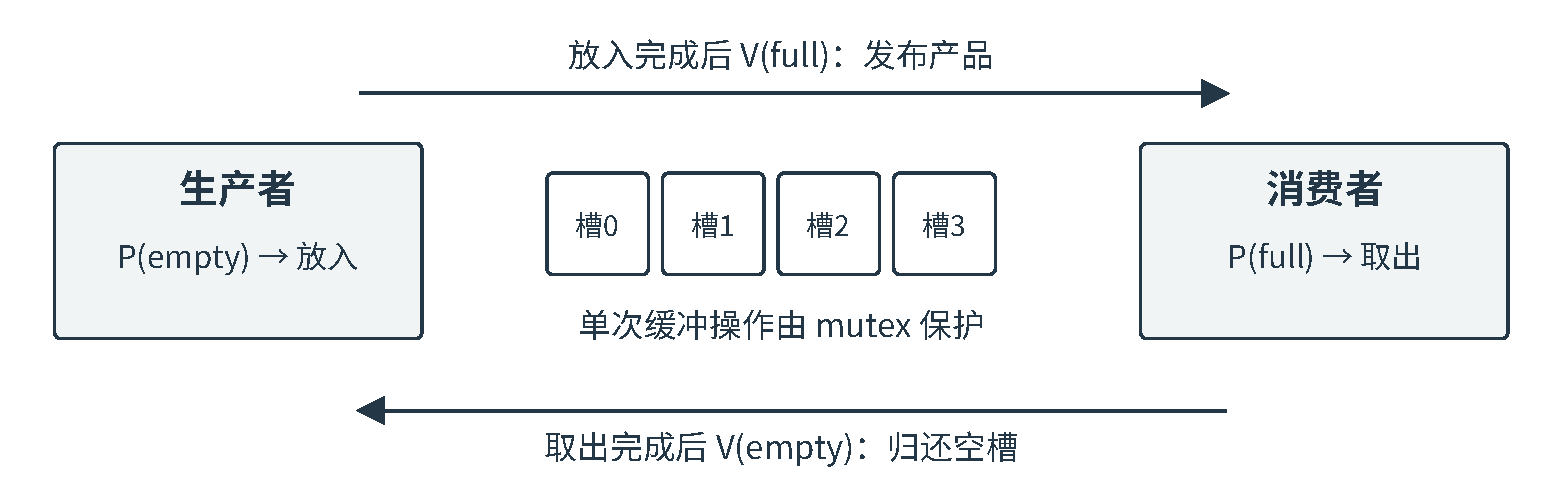
\includegraphics[width=\linewidth,height=125mm,keepaspectratio]{figures/F04_buffer_permissions.pdf}
\captionof{figure}{空位许可与产品许可沿相反方向流动；四个槽只是示意，算法容量仍为 n}\label{fig-buffer}
\end{minipage}\par\medskip

\BlueLines{4,6,7}
\begin{codeblock}[language={}]
semaphore empty = n, full = 0, mutex = 1;

producer() {
    while (true) {
        x = produce();
        P(empty);          // 先取得一个空槽许可
        P(mutex);
        put(x);
        V(mutex);
        V(full);           // 放入完成，才能发布产品
    }
}
\end{codeblock}

\BlueLines{2,3,4}
\begin{codeblock}[language={}]
consumer() {
    while (true) {
        P(full);           // 先取得一个产品许可
        P(mutex);
        x = get();
        V(mutex);
        V(empty);
        consume(x);
    }
}
\end{codeblock}

``尚未被申请''这一限定不能省略。容量为 2、初始为空时，一个生产者刚执行 P(empty) 而尚未放入，\texttt{empty=\allowbreak{}1,\allowbreak{} full=\allowbreak{}0}，物理空槽却仍有 2 个。空槽已预留，信号量先减少，实际空位数还没变；消费者取得 \texttt{full} 后、实际取出前也类似。因此，执行中每一步的 \texttt{empty+\allowbreak{}full} 都未必等于 \(n\)，\texttt{full} 也未必等于实存产品数。只有两个计数均非负，且既无已取得但尚未使用的许可、也无操作完成却尚未发布的许可时，才能把它们分别与物理空槽数、产品数对照。计数为负时，其绝对值表示相应等待者数。

\subsubsection{为什么不能持有缓冲区锁等待产品}\label{OS02-auto-16}

若消费者先 \texttt{P(\allowbreak{}mutex)\allowbreak{}} 再 \texttt{P(\allowbreak{}full)\allowbreak{}}，初始为空时，它会持锁阻塞。生产者随后申请 \texttt{mutex} 也阻塞；消费者等生产者放入，生产者等消费者解锁，形成等待环。

\par\medskip\noindent\begin{minipage}{\linewidth}
\centering
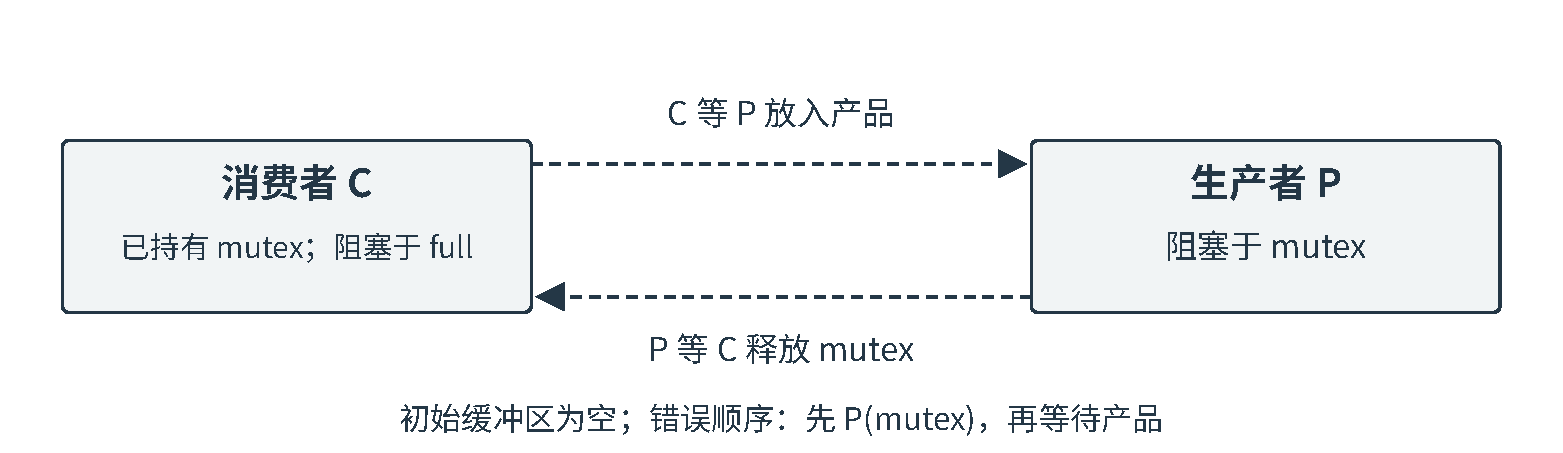
\includegraphics[width=\linewidth,height=125mm,keepaspectratio]{figures/F05_buffer_deadlock.pdf}
\captionof{figure}{错误的 P 顺序使能够改变条件的进程也被挡住}\label{fig-deadlock}
\end{minipage}\par\medskip

所以在这个算法中，容量或产品的 P 在外，缓冲区锁的 P 在内。判断别的算法时仍要追问：当前持有什么，等待什么，谁能使条件成立，对方是否也要用所持资源。不能把``同步 P 总在所有互斥 P 前''当成普遍定理；\hyperref[OS02-ex-2014]{整批取数}和\hyperref[OS02-readers]{读者组}会给出更具体的锁范围。

放入之后，本算法的 \texttt{V(\allowbreak{}mutex)\allowbreak{}} 与 \texttt{V(\allowbreak{}full)\allowbreak{}} 可交换：消费者即使先收到产品许可，仍须取得 \texttt{mutex} 才能取出。原顺序可避免提前唤醒后再等锁。这个判断依赖放入已经完成、且后续访问也持锁；不是所有 V 都能任意挪动。

〖2.3-039〗 生产者---消费者模型处理的是进程之间的同步与互斥。它本身不保证公平；错误的 P 顺序还可能制造死锁。避免这一错误顺序只是正确实现的必要条件，不能据此声称该模型能解决任意死锁。

\subsubsection{例 2B-5　消费者只能取特定类别时怎样计数}\label{OS02-ex-2009}

\begin{example}[配套例题]

【配套例题】 三个进程 P1、P2、P3 互斥使用一个包含 N（N\textgreater0）个单元的缓冲区。P1 每次用 produce() 生成一个正整数并用 put() 送入缓冲区某一空单元中；P2 每次用 getodd() 从该缓冲区中取出一个奇数并用 countodd() 统计奇数个数；P3 每次用 geteven() 从该缓冲区中取出一个偶数并用 counteven() 统计偶数个数。请用信号量机制实现这三个进程的同步与互斥活动，并说明所定义信号量的含义（要求用伪代码描述）。

\end{example}

\textbf{解析。} ``缓冲区非空''不足以允许 P2 取数：其中可能只有偶数。保留共同的空位许可，把产品许可按可取条件拆为 \texttt{odd} 与 \texttt{even}；三种缓冲操作共用 \texttt{mutex}。

原题未明说缓冲区初态。以下按参考答案采用\textbf{初始为空}：\texttt{empty=\allowbreak{}N,\allowbreak{} odd=\allowbreak{}even=\allowbreak{}0,\allowbreak{} mutex=\allowbreak{}1}。令 \texttt{x} 是 P1 本次生成的本地整数，\texttt{put(\allowbreak{})\allowbreak{}} 放入它；保留题设函数名。

\BlueLines{4,6,7}
\begin{codeblock}[language={}]
semaphore empty = N, odd = 0, even = 0, mutex = 1;

P1() {
    while (true) {
        x = produce();
        P(empty);
        P(mutex);
        put();
        V(mutex);
        if (x % 2 != 0) V(odd); else V(even);
    }
}
\end{codeblock}

\BlueLines{2,3,4}
\begin{codeblock}[language={}]
P2() {
    while (true) {
        P(odd);
        P(mutex);
        getodd();
        V(mutex);
        V(empty);
        countodd();
    }
}
\end{codeblock}

\BlueLines{2,3,4}
\begin{codeblock}[language={}]
P3() {
    while (true) {
        P(even);
        P(mutex);
        geteven();
        V(mutex);
        V(empty);
        counteven();
    }
}
\end{codeblock}

每次 put 只发布所放入的产品所属类别的一份许可，消费者不能拿另一类别的许可代用。getodd/geteven 完成后，空位可立刻交还；各自的统计不访问共享缓冲区，留在锁外。

若初始已有 \(a\) 个奇数、\(b\) 个偶数，则应改为 \texttt{odd=\allowbreak{}a,\allowbreak{} even=\allowbreak{}b,\allowbreak{} empty=\allowbreak{}N-a-b}，其中 \(a,b\ge0\) 且 \(a+b\le N\)。若长期没有某类别的产品产出，该类别的消费者就可能持续等待，直到该类产品出现；只要生产者和另一消费者仍前进，就不能仅凭这一等待认定系统死锁。题目没有保证所有类别都会出现。

\subsubsection{例 2B-6　连续取 10 件改变的是哪一层互斥}\label{OS02-ex-2014}

\begin{example}[配套例题]

【配套例题】 系统中有多个生产者进程和多个消费者进程，共享一个能存放 1000 件产品的环形缓冲区（初始为空）。当缓冲区未满时，生产者进程可以放入其生产的一件产品，否则等待；当缓冲区未空时，消费者进程可以从缓冲区取走一件产品，否则等待。要求一个消费者进程从缓冲区连续取出 10 件产品后，其他消费者进程才可以取产品。请使用信号量 P、V（或 wait()、signal()）操作实现进程间的互斥与同步，要求写出完整的过程，并说明所用信号量的含义和初值。

\end{example}

\textbf{解析。} ``连续''限制其他消费者插入取数，不禁止生产者在这期间补货。由此需要两个范围：\texttt{mutex=\allowbreak{}1} 保护一次缓冲操作，\texttt{batch=\allowbreak{}1} 由一个消费者持有直到它取满 10 件。生产者不申请 \texttt{batch}。

\BlueLines{6,8,9}
\begin{codeblock}[language={}]
semaphore empty = 1000, full = 0, mutex = 1, batch = 1;
item buf[1000];
int in = 0, out = 0;

producer() {
    while (true) {
        x = produce();
        P(empty);
        P(mutex);
        buf[in] = x;
        in = (in + 1) % 1000;
        V(mutex);
        V(full);
    }
}
\end{codeblock}

\BlueLines{2,3,5}
\begin{codeblock}[language={}]
consumer() {
    while (true) {
        P(batch);
        for (int k = 0; k < 10; ++k) {
            P(full);
            P(mutex);
            local[k] = buf[out];
            out = (out + 1) % 1000;
            V(mutex);
            V(empty);
        }
        V(batch);
        consume(local);
    }
}
\end{codeblock}

\texttt{empty}、\texttt{full} 的含义与初值来自容量和初态。\texttt{in/\allowbreak{}out} 分别指向下一次放入、取出的位置；\texttt{local[0..9]} 是消费者私有的十件产品存储。每次取走一件就归还一个空槽，不必等整批结束。

假设消费者已取出 3 件，缓冲区暂时为空。它持有 \texttt{batch}，等 \texttt{full}；但它没有持有 \texttt{mutex}，生产者能继续放入并 V(full)，因此可接着取第 4 件。其他消费者不能插入，所要求的连续性得到保持。若把 \texttt{mutex} 从整批开头一直持有到末尾，消费者会在缺货时挡住补货者，形成死锁。

本解不要求开始时凑齐 10 件。不要让多个消费者在批锁之外各申请若干产品许可，再等凑够十个；这会把产品预留给多个消费者，破坏整批协调。\texttt{batch} 在前并非违反上一节的锁顺序：真正要检查的是生产者是否也依赖它，以及消费者等待产品时是否仍给生产者留下执行通路。

\subsection{多个读者怎样作为一组申请资源}\label{OS02-readers}

读者---写者模型允许多个读者同时读共享文件；写者之间互斥，写者与任何读者互斥。读者读完不清空文件，因此``已有数据''不应被当作一个被读走就消耗的产品许可。以下采用王道书 §2.3 的经典模型；每次读或写的时间有限，所有访问者遵守同一协议。

\subsubsection{首读者申请，末读者释放}\label{OS02-auto-17}

令 \texttt{rw=\allowbreak{}1} 表示文件访问权：一个写者独占，或者一组读者共同持有。共享计数 \texttt{readCount=\allowbreak{}0} 记录已登记但尚未退出的读者数，\texttt{countMutex=\allowbreak{}1} 保护该计数和首末读者判断。

\BlueLines{5,6,8}
\begin{codeblock}[language={}]
semaphore rw = 1, countMutex = 1;
int readCount = 0;

reader() {
    P(countMutex);
    if (readCount == 0) P(rw);
    readCount++;
    V(countMutex);

    读文件;

    P(countMutex);
    readCount--;
    if (readCount == 0) V(rw);
    V(countMutex);
}
\end{codeblock}

\BlueLines{2,4}
\begin{codeblock}[language={}]
writer() {
    P(rw);
    写文件;
    V(rw);
}
\end{codeblock}

第一个读者为整组取得 \texttt{rw}，后续读者只登记，不重复申请 \texttt{rw}；最后一个读者离开才归还。若每个读者都在读文件前 P(rw)、读后 V(rw)，读者也被串行化，题目允许的并发便丢失了。

\par\medskip\noindent\begin{minipage}{\linewidth}
\centering
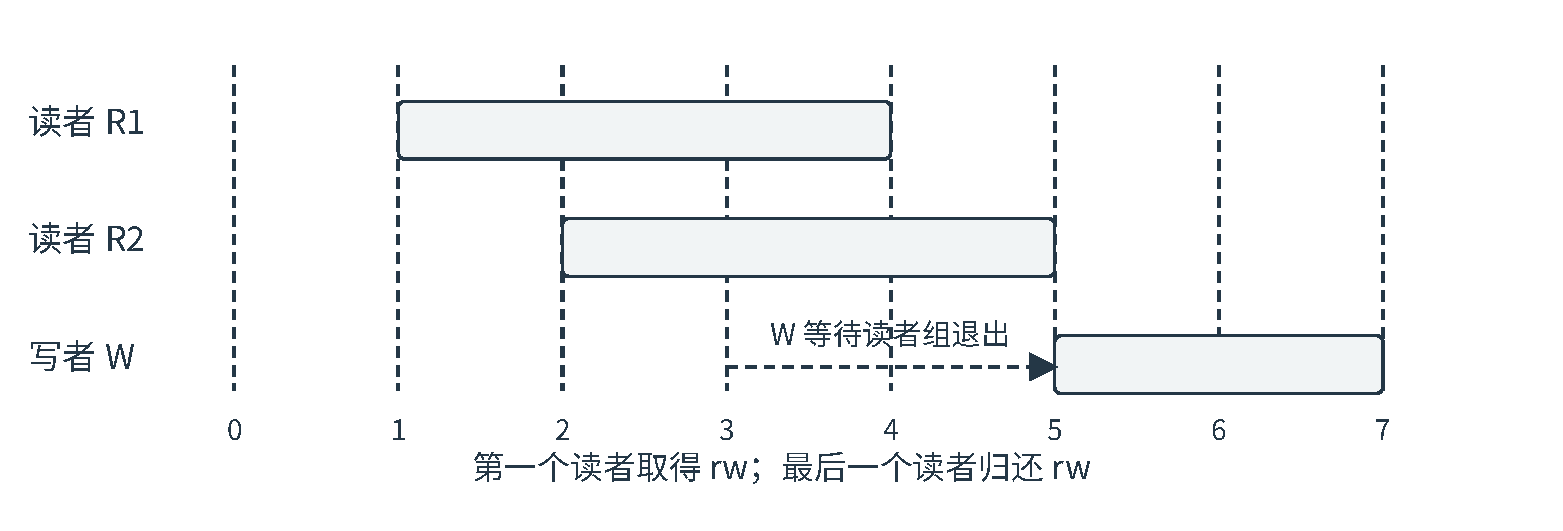
\includegraphics[width=\linewidth,height=125mm,keepaspectratio]{figures/F06_readers_group.pdf}
\captionof{figure}{重叠的两个读者共同占有一个读者组的文件访问权；横轴为示意时间}\label{fig-readers}
\end{minipage}\par\medskip

计数的检查和修改须在同一个受保护范围。假设只保护加减、不保护前面的判断：\texttt{readCount=\allowbreak{}1} 时，新读者检查到非零，准备跳过 P(rw)，此时暂停；原有的最后一个读者退出，把计数减到 0 并释放 rw；写者取得 rw 后，新读者才恢复，将计数加 1 并开始读。新读者没有申请 rw，却与写者同时访问。把判断和登记一起保护，才能排除这条交错。

首读者可能持有 \texttt{countMutex} 等待 \texttt{rw}，此处为何不必然死锁？它等待时 \texttt{readCount=\allowbreak{}0}，所以没有已登记的读者需要取得 \texttt{countMutex} 来做末读者退出；正在写的进程归还 \texttt{rw} 也不需要 \texttt{countMutex}。

\subsubsection{读者优先与公平需要分别说明}\label{OS02-auto-18}

上述算法中，只要仍有读者在读，新来的读者就能加入同一组，即使已有写者等 \texttt{rw}。不断到来的读者可能使 \texttt{readCount} 始终不归零，写者因而饥饿。

一种改法是加入口信号量 \texttt{gate=\allowbreak{}1}。每个读者在登记前 P(gate)，登记后 V(gate)；写者则 P(gate)、P(rw)，写完后依次 V(rw)、V(gate)。其余读者退出代码不变：

\BlueLines{2,3,4}
\begin{codeblock}[language={}]
// 读者的入口，替换上一算法的入口部分
P(gate);
P(countMutex);
if (readCount == 0) P(rw);
readCount++;
V(countMutex);
V(gate);

// 写者完整过程
P(gate);
P(rw);
写文件;
V(rw);
V(gate);
\end{codeblock}

一旦写者取得 \texttt{gate}，新读者不能再登记；原有读者仍能按原退出代码离开，最后一个释放 \texttt{rw}，写者便可进入。若 \texttt{gate} 队列按先进先出服务，且进程持续获得执行机会、每次读写有限，可进一步说明等待者不会被后来者无限越过。\textbf{仅有信号量而没有公平排队约定，不能无条件宣称``不会饥饿''或``严格先来先服务''。} 它也不是绝对的写优先策略：写者并不在任何到达次序下都先于读者进入。

\subsection{哲学家进餐：申请多个资源时怎样断开等待环}\label{OS02-philosophers}

五个哲学家 \(P_0\) 至 \(P_4\) 围桌而坐，每人须同时持有左右两根筷子才能吃饭。一根筷子只供一人使用，吃完归还，再思考。统一编号：\(P_i\) 需要 \(C_i\) 与 \(C_{(i+1)\bmod5}\)，每个筷子信号量初值为 1。经典模型见王道书 §2.3。

如果所有人都先 P(C{[}i{]}) 再 P(C{[}(i+1)\%5{]})，一种允许的交错是每人先拿到一根。此时每人都在等右邻已经拿着的那一根，无人能到达归还步骤。

\par\medskip\noindent\begin{minipage}{\linewidth}
\centering
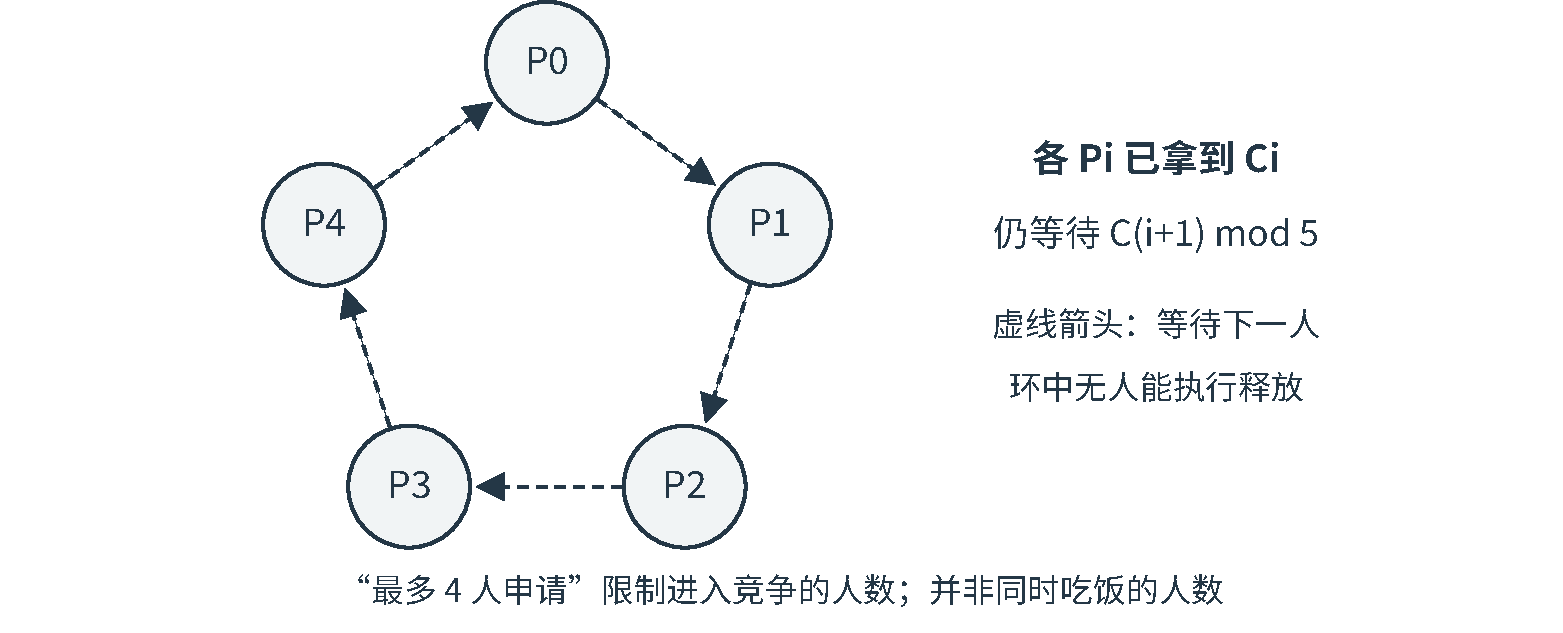
\includegraphics[width=\linewidth,height=125mm,keepaspectratio]{figures/F07_philosopher_wait_cycle.pdf}
\captionof{figure}{每个进程只持有一根筷子，也足以形成整体死锁}\label{fig-philosophers}
\end{minipage}\par\medskip

\subsubsection{限制竞争人数，与限制同时吃饭人数不同}\label{OS02-auto-19}

增加 \texttt{room=\allowbreak{}4}，使最多四人处在``开始拿筷子到全部归还''的区间内：

\BlueLines{5,7,8}
\begin{codeblock}[language={}]
semaphore room = 4;
semaphore C[5] = {1, 1, 1, 1, 1};

philosopher(i) {
    while (true) {
        思考;
        P(room);
        P(C[i]);
        P(C[(i+1) % 5]);
        吃饭;
        V(C[(i+1) % 5]);
        V(C[i]);
        V(room);
    }
}
\end{codeblock}

若所有竞争者都各持一根并等待下一根，要形成完整环就必须五人都参与；\texttt{room=\allowbreak{}4} 阻止了这种状态。沿等待方向追下去，要么遇到一根还没被占用的筷子，要么遇到正在吃饭、能够归还筷子的人。只要持有者继续执行、进餐有限，就不会陷入上述整体等待环。

这里的 4 是同时申请区间内的人数上限。五根筷子最多支持 \(\lfloor5/2\rfloor=2\) 人同时吃饭，不能把``最多四人申请''误读为``四人同时进餐''。该办法排除了这种死锁情形，但并不保证某个饥饿者最终抢到许可；仍需公平条件。

另一种办法是全局排序：所有人都先取编号较小、再取较大的筷子。若存在资源等待环，沿环等待的资源编号就必须严格递增，最后又回到起点，不可能成立。每人独立``先左后右''不是全局排序；编号相邻位置在取模后更须检查。

也可用额外互斥量把``拿两根''的过程串行化，拿齐后立即释放这个额外量，吃完直接归还筷子。这能断开多人各拿一根的环，但可能让一个正在等筷子的人挡住另一个本可拿齐的人。它也不等于``先原子检查两根都空闲，然后同时取得''；若题目要求整组资源同时分配，就需要更强的原子检查与分配机制。

\subsection{管程与条件变量：等待时必须让出改变条件的机会}\label{OS02-monitor}

\textbf{管程}把共享数据、对数据的操作过程和初始化封装在一个同步模块中，参与者通过规定的入口访问这些数据；同一时刻至多一个进程在其中执行。这个互斥规则由实现管程的语言或运行系统保证，不要求调用者在每个入口外重复编写 P、V。管程不是一个自行运行的进程。

但``每次只准一人进入''还不够：消费者进入后可能发现无产品。若它在管程里循环等待并一直保有管程，生产者就无法进入改变条件。\textbf{条件变量}为这种等待提供队列；实际条件由共享数据上的布尔判断表达，例如 \texttt{count>\allowbreak{}0}。条件变量本身不是保存产品数的整数。

\subsubsection{wait 负责等待，不替调用者判断条件}\label{OS02-auto-20}

\subsubsection{例 2B-7　条件变量的 wait 做什么}\label{OS02-ex-2018}

\begin{example}[配套例题]

【配套例题】 若 x 是管程内的条件变量，则当进程执行 x.wait() 时所做的工作是（　）。

A. 实现对变量 x 的互斥访问

B. 唤醒一个在 x 上阻塞的进程

C. 根据 x 的值判断该进程是否进入阻塞态

D. 阻塞该进程，并将之插入 x 的阻塞队列中

\end{example}

答案为 \textbf{D}。调用者先检查共享状态，只有需要等待时才调用 x.wait()；调用后进入 x 的等待队列，并释放管程使用权，让其他进程能进入。C 把``调用前的条件判断''放进了 wait 的职责，还把 x 当作可直接取值的资源计数。

管程中执行 x.signal()，是通知一个已经在 x 上等待的进程。若没有等待者，通知不积累；以后进入的进程须重新检查共享状态。信号量 V 即使没有等待者，也会使计数增加，留下一个可供后续 P 使用的许可。

〖2.3-029〗 ``管程中 signal 操作的作用和信号量机制中的 V 操作相同''不成立。检查无等待者的边界即可区分：前者不留下通知，后者增加许可。管程作为同步模块，与一个可独立运行的进程也不是同一类对象；具体语言的管程对象能否实例化，应由语言规定。

\subsubsection{通知以后，何时重新检查条件}\label{OS02-auto-21}

不同管程定义对 signal 后的运行次序有不同规定。Hoare 式语义可立即转交管程给被唤醒者；Mesa 式语义让通知者继续，等待者以后重新竞争进入权。题目若给出特定语义，应据此推演，不能混用。

下面用 Mesa / POSIX 式条件等待说明可独立执行的做法。\texttt{wait(\allowbreak{}cv,\allowbreak{}m)\allowbreak{}} 把释放互斥锁 m 与进入等待合并为一个原子操作；返回前重新取得 m。通知不保证等待者马上运行，也不保证等它重新取得 m 时条件仍成立，所以用 \texttt{while} 重检。实际接口还可能出现虚假唤醒，同样需要重检。

\par\medskip\noindent\begin{minipage}{\linewidth}
\centering
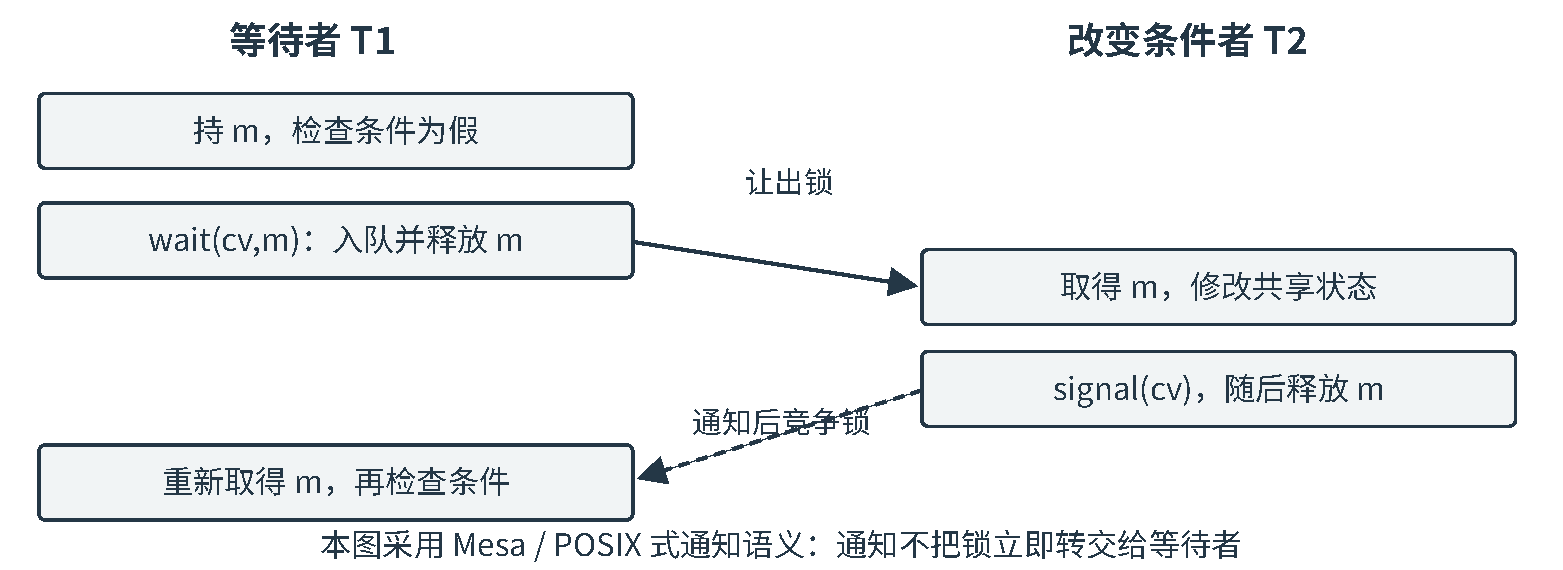
\includegraphics[width=\linewidth,height=125mm,keepaspectratio]{figures/F08_condition_wait.pdf}
\captionof{figure}{wait 释放锁，使另一个线程能够改变共享状态；等待返回前须重新取得锁}\label{fig-monitor}
\end{minipage}\par\medskip

设这个模块的容量为 \(n>0\)，初始为空，m 初始化为未加锁；插入和取出维护同一个缓冲区。

\BlueLines{8}
\begin{codeblock}[language={}]
// 单个缓冲模块的共享状态
mutex m;
condition notEmpty, notFull;
int count = 0;

put(x) {
    lock(m);
    while (count == n) wait(notFull, m);
    插入 x; count++;
    signal(notEmpty);
    unlock(m);
}
\end{codeblock}

\BlueLines{3,7}
\begin{codeblock}[language={}]
get() {
    lock(m);
    while (count == 0) wait(notEmpty, m);
    x = 取出元素; count--;
    signal(notFull);
    unlock(m);
    return x;
}
\end{codeblock}

若消费者发现空就调用 wait，它释放 m；生产者才能取得 m 放入，并通知消费者。被通知者回来时再次检查 \texttt{count}，是因为这期间可能已有另一个消费者先取走产品。不能把 \texttt{wait} 拆成普通的``先 unlock，再单独入队''：另一线程可能恰在两步之间发出无人接收的通知，等待者随后入队，就错过了这次机会。

这里的接口语义用于把等待机制讲清，并非要求记忆 POSIX 参数及错误码。参见 The Open Group《Base Specifications Issue 8》条件等待与通知条目；管程概念与条件变量的比较见王道书 §2.3。

\subsection{写出并发代码后，怎样检验}\label{OS02-method}

题干中的名词不会直接决定信号量个数。先把每个进程的一次活动写清，标出它开始前必须成立的条件，再说明谁能使该条件成立。把``可用槽位''``某类产品''``阶段已经完成''等条件转成许可，把会冲突的共享状态操作放进相应互斥范围，才能确定变量及初值。

\begin{wideblock}

\par\medskip\noindent\begin{minipage}{\linewidth}\fontsize{9.3}{12}\selectfont\begin{tabularx}{\linewidth}{@{}YYY@{}}
\toprule\noalign{}
\begin{minipage}[b]{\linewidth}\raggedright
题干给出的条件
\end{minipage} & \begin{minipage}[b]{\linewidth}\raggedright
转成什么关系
\end{minipage} & \begin{minipage}[b]{\linewidth}\raggedright
应检查的代码位置
\end{minipage} \\
\midrule\noalign{}


必须等某操作完成 & 完成通知，初值由该事件是否已发生决定 & 前操作完成后 V，后操作开始前 P。 \\
最多容纳 n 件 & 容量许可，有放入与归还两个方向 & 先申请空位，放入后发布产品，取出后归还空位。 \\
只能取某一类 & 每一类独立的可取条件 & 发布对应类别，不以总的 full 代替各类别许可。 \\
多个读者可以并行 & 读者组与写者互斥 & 保护首末读者判断，而非将整个读操作串行化。 \\
连续取 k 件后才轮到别人 & 消费者整批排他 & 批锁覆盖 k 次，缓冲锁只覆盖单次；等待时允许补货。 \\
\bottomrule\end{tabularx}
\end{minipage}\par\medskip

\end{wideblock}

最后手推几条会暴露错误的轨迹：后继先运行、缓冲区初始为空或已满、两个请求几乎同时到达、一个进程拿到许可但尚未实际操作、通知发出但被通知者尚未重新运行。每一步记下``持有---等待---可执行者''。检查安全性后，再分别检查死锁、饥饿与不必要的串行化；三者不能互相代替。

\subsection{分支自测：先判断，再看答案}\label{OS02-selfcheck}

原创回顾设问：下列问题依据本章例题与经典模型编写，用于检查中间状态和适用边界。

\begin{enumerate}
\def\labelenumi{\arabic{enumi}.}
\tightlist
\item
  按\hyperref[OS02-semaphore]{记录型语义}，P 前 \texttt{S.value=\allowbreak{}1}，P 后为 0，要阻塞吗？一次 V 使值从 \ensuremath{-}1 变为 0，要唤醒吗？被唤醒者是否还要为这次申请再减 1？
\item
  在\hyperref[OS02-ex-2022]{前驱题}中，能否在 D 完成后才 signal(S\_CE)？这样是否保留了图允许的所有并发？
\item
  在\hyperref[OS02-ex-2009]{分类缓冲题}中，初态有 \(a\) 个奇数、\(b\) 个偶数，三个计数信号量怎样初始化？如果缓冲区只有偶数，P2 等待能否说明整个系统死锁？
\item
  在\hyperref[OS02-ex-2014]{成批取数题}中，某消费者取了 3 件后暂时缺货，应继续持有哪个量、等待哪个量？生产者还能否运行？
\item
  哲学家最多允许四人进入申请区，是否能有四人同时吃饭？
\item
  条件变量 signal 在没有等待者时，是否留下一份以后可取得的许可？
\end{enumerate}

\subsubsection{自测答案}\label{OS02-auto-22}

\begin{enumerate}
\def\labelenumi{\arabic{enumi}.}
\tightlist
\item
  P 后为 0 不阻塞，表示取走最后一个许可。V 后为 0 仍须唤醒一个等待者；它已取得本次申请的机会，不再为同一次 P 减 1。
\item
  能保证 E 不早于 C，却额外让 E 等 D，缩小并发范围。通知应在 C 完成后、D 前发出。
\item
  \texttt{empty=\allowbreak{}N-a-b,\allowbreak{} odd=\allowbreak{}a,\allowbreak{} even=\allowbreak{}b}；需 \(a,b\ge0\)、\(a+b\le N\)。若只有 P2 无奇数可取，不能推出整个系统无法前进。
\item
  持有 \texttt{batch}、等待 \texttt{full}，此时没有持有 \texttt{mutex}。生产者不需要 \texttt{batch}，仍能取得空位与缓冲区锁，补入产品。
\item
  最多两人同时吃饭，四是申请区间内的人数上限。
\item
  条件变量通知不积累为以后可消费的许可；有资源初态要用共享状态表达。
\end{enumerate}

条件变量等待语义另参 The Open Group 条件等待与通知接口、Oracle《Using Condition Variables》。

\section{死锁：从资源分配状态判断能否继续}\label{OS02-module-04}

进程因为得不到资源而等待，并不一定发生死锁。要判断是否会死锁，还需追问：谁持有该进程所需的资源，持有者能否完成并归还，归还又依赖谁。本章把这种追踪分别用于死锁条件、资源分配图、安全检查和死锁检测。

除特别说明，讨论的是可重复使用的资源：每类可以有多个同类实例，资源只能在释放后再次分配；进程请求后若不能满足便等待，正常完成会归还已持资源。分析安全性还假定进程声明的最大需求可信，不超过系统允许的资源总量，并能在获得所需资源后有限完成。

\subsection{死锁、饥饿和不安全状态}\label{OS02-4-1}

\textbf{死锁}指一组进程中，每个进程都在等待一个只能由组内进程引起的事件（其中也包括自身尚未执行的释放动作），因而这一组无法自行推进。最小的双资源例子是：P 持有 A 等 B，Q 持有 B 等 A；没有进程能到达释放步骤。

\textbf{饥饿}指某个进程长期得不到所需服务，而其他进程仍可能持续前进。例如读者不断加入，使写者一直拿不到写权限。\textbf{死循环}是执行路径自身不能结束，进程可能仍持续占用 CPU，不必等待其他进程。三者的机制不同，处理方法也不同。

\subsubsection{四个必要条件是同时约束}\label{OS02-auto-23}

\begin{wideblock}

\par\medskip\noindent\begin{minipage}{\linewidth}\fontsize{9.3}{12}\selectfont\begin{tabularx}{\linewidth}{@{}YYY@{}}
\toprule\noalign{}
\begin{minipage}[b]{\linewidth}\raggedright
条件
\end{minipage} & \begin{minipage}[b]{\linewidth}\raggedright
本章资源模型中的含义
\end{minipage} & \begin{minipage}[b]{\linewidth}\raggedright
怎样在状态中识别
\end{minipage} \\
\midrule\noalign{}


互斥 & 某类实例同一时刻只能给一个进程使用 & 资源不可被两个申请者同时使用 \\
占有并等待 & 保持已有资源，同时等待新增资源 & 一个进程既有分配边，又有请求边 \\
不可剥夺 & 未用完的资源不能被系统任意收回 & 只能由持有者按规则释放 \\
循环等待 & 存在首尾相接的资源等待链 & P 等 Q，Q 又直接或间接等 P \\
\bottomrule\end{tabularx}
\end{minipage}\par\medskip

\end{wideblock}

发生这类资源死锁时，四项同时成立；只满足其中一项或几项不能推出死锁。``四项必要条件都允许存在''也不等于任何时刻都已经死锁，还要检查实际持有与等待状态。单进程再次请求一个自己已经持有且不可重入的锁，也可能自我阻塞，不能把``死锁至少要两个进程''当作适用于所有锁语义的结论。

\subsubsection{资源分配图中的环什么时候足够}\label{OS02-auto-24}

进程用圆表示，资源类型用方框表示，框内点表示实例。\(P_i\to R_j\) 是请求边，\(R_j\to P_i\) 是一个实例的分配边。没有有向环，可排除这种资源等待死锁；有环时，若环中相关资源类型均只有一个实例，则可判定死锁。

若资源类型有多个实例，环只说明可能死锁。例如 P 持有 A 的一个实例、等待 B，Q 持有 B、等待 A，但 A 还有一个空闲实例，Q 取得它并完成后就能释放 B。图中已有等待环，却仍有解开它的执行通路。此时必须结合实例数化简或执行检测算法。

\par\medskip\noindent\begin{minipage}{\linewidth}
\centering
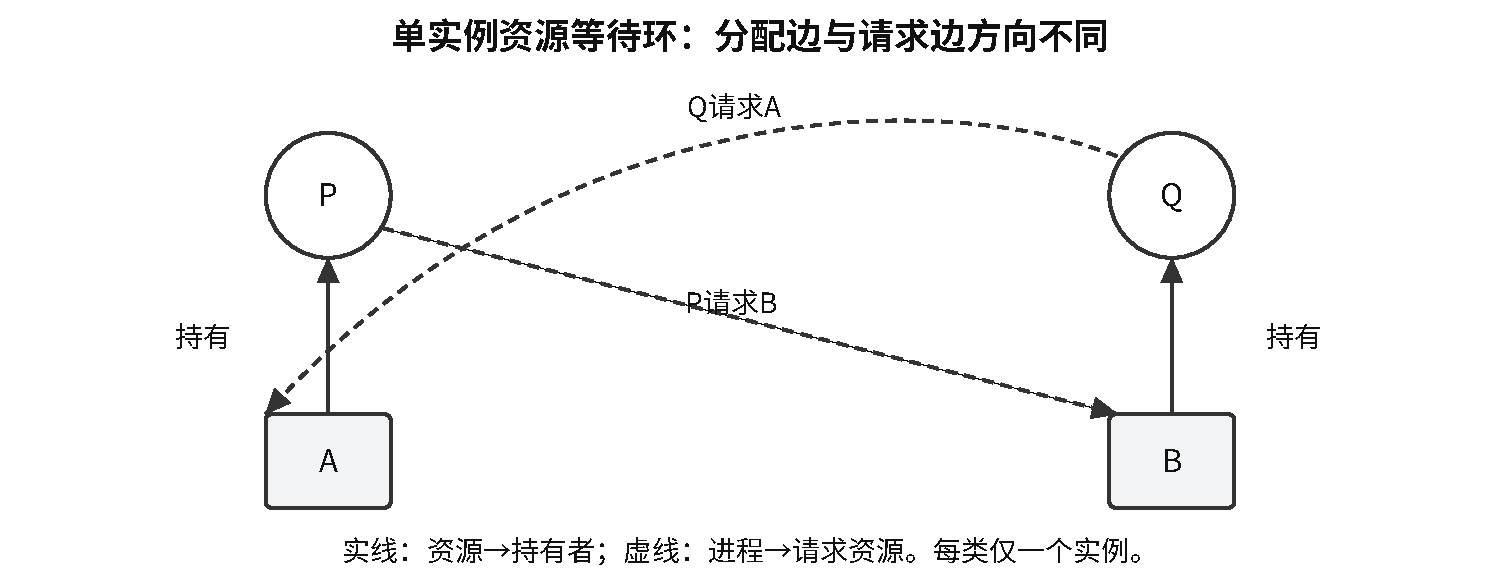
\includegraphics[width=\linewidth,height=125mm,keepaspectratio]{figures/OS_resource_graph.pdf}
\captionof{figure}{单实例环中每个人都等别人；增加可用实例后必须重新检查能否推进}\label{os-fig-resource}
\end{minipage}\par\medskip

\subsubsection{安全状态问的是``能否保证全部完成''}\label{OS02-auto-25}

\textbf{安全序列}是进程的一种次序，使每个进程在轮到它时，现有可用资源加上此前已完成进程释放的资源，足以满足它尚需的最大资源量。若存在至少一个安全序列，则称当前状态安全。

安全状态并不意味着系统只能按这一序列运行；该序列是可完成性的证据。\textbf{不安全}表示无法在最大需求假设下给出这样的保证，不代表此刻已经死锁。进程可能还没提出全部需求，也可能实际少用资源或提前释放。死锁状态必不安全；不安全状态可能在以后的某种申请序列中发展成死锁。

\subsection{死锁预防：在规则中破坏一个条件}\label{OS02-4-2}

\textbf{预防}是在分配规则上使至少一个必要条件不能成立，不必等到死锁已经出现。

让可共享的资源按共享方式使用，可以去掉相应的互斥条件；但打印机输出、独占锁等具有不可共享的语义，不能为了避免死锁而取消必要保护。一次性申请运行所需的全部资源，全部满足才开始，可以破坏占有并等待，但会降低利用率，并要求提前知道需求。申请失败时先释放已有资源再重试，也是破坏``占有并等待''的办法。

对可保存、恢复状态的资源，可以在适当时机剥夺并回滚，例如某些处理器或存储资源；正在打印到纸张上的半份输出却不能简单撤回。对所有资源规定统一编号，只允许按严格递增次序申请，可以破坏循环等待：若有环，沿环的资源编号必须不断增大又回到起点，无法成立。各进程都只按``先拿左边、再拿右边''申请，并不等于有了统一的全局编号，仍可能形成环。

预防可能限制请求方式并造成资源闲置。\textbf{避免}则保留更多请求自由，在每次拟分配时检查分配后的状态是否仍然安全。二者都在实际进入死锁前采取措施，但依据不同。

\subsubsection{例 2C-1　避免与检测需要的信息不同}\label{OS02-ex4-1}

\begin{example}[配套例题]

【配套例题】 若系统 S1 采用死锁避免方法，S2 采用死锁检测方法。下列叙述中，正确的是（　）。

\ensuremath{\mathrm{I}}. S1 会限制用户申请资源的顺序，而 S2 不会

\ensuremath{\mathrm{II}}. S1 需要进程运行所需的资源总量信息，而 S2 不需要

\ensuremath{\mathrm{III}}. S1 不会给可能导致死锁的进程分配资源，而 S2 会

A. 仅\ensuremath{\mathrm{I}}、\ensuremath{\mathrm{II}}　　B. 仅\ensuremath{\mathrm{II}}、\ensuremath{\mathrm{III}}　　C. 仅\ensuremath{\mathrm{I}}、\ensuremath{\mathrm{III}}　　D. \ensuremath{\mathrm{I}}、\ensuremath{\mathrm{II}}、\ensuremath{\mathrm{III}}

\end{example}

\textbf{解析。} 银行家算法这类避免方法根据最大需求和当前状态决定批准还是推迟，并不规定所有进程必须按统一资源顺序申请；\ensuremath{\mathrm{I}}混入了预防中的资源有序分配法。避免要判断未来最大需求是否仍可满足；检测根据当前已分配与当前等待请求判断，不要求事先掌握全过程最大需求。检测允许某些分配在以后导致死锁，事后再检测并解除。因此\ensuremath{\mathrm{II}}、\ensuremath{\mathrm{III}}正确，答案为 \textbf{B}。

\subsection{银行家算法：可用不等于可以批准}\label{OS02-4-3}

设有 \(n\) 个进程、\(m\) 类资源。向量按同一资源次序排列，各分量逐项比较，不能用向量元素之和代替比较。

\begin{wideblock}

\par\medskip\noindent\begin{minipage}{\linewidth}\fontsize{9.3}{12}\selectfont\begin{tabularx}{\linewidth}{@{}YY@{}}
\toprule\noalign{}
名称 & 含义 \\
\midrule\noalign{}


\texttt{Available[j]} & 第 j 类当前未分配的实例数 \\
\texttt{Max[i][j]} & 进程 i 声明的第 j 类最大需求 \\
\texttt{Allocation[i][j]} & 进程 i 已持有的实例数 \\
\texttt{Need[i][j]} & 进程 i 尚可能需要的最大数量，等于 \texttt{Max-Allocation} \\
\bottomrule\end{tabularx}
\end{minipage}\par\medskip

\end{wideblock}

\subsubsection{安全性检查中的 Work 为什么要加 Allocation}\label{OS02-auto-26}

先复制 \texttt{Work=\allowbreak{}Available}，所有 \texttt{Finish=\allowbreak{}false}。反复寻找未完成且 \texttt{Need[i] <\allowbreak{}=\allowbreak{} Work} 的进程：假定给足它的剩余需求，它完成后会归还所有资源，净效果是 \texttt{Work +\allowbreak{}=\allowbreak{} Allocation[i]}，并标记完成。若最终所有进程都能标记，则安全；若再无可选者但仍有未完成者，则不安全。

之所以只加原 \texttt{Allocation}，是因为假定借给它的 \texttt{Need} 已从 Work 中暂时扣掉，完成时又随资源归还，二者相抵。若把 \texttt{Max} 直接加到 Work，就会凭空增加资源；若把 Work 逐步减到负数，再说``以后会归还''，则跳过了本算法的可完成前提。

\BlueLines{3}
\begin{codeblock}[language={}]
Work = Available
Finish[0..n-1] = false
while 存在 i: !Finish[i] 且 Need[i] <= Work:
    Work = Work + Allocation[i]
    Finish[i] = true
若全部 Finish 为真，则安全；否则不安全
\end{codeblock}

\subsubsection{例 2C-2　能先完成两人，仍然可能不安全}\label{OS02-ex4-2}

\begin{example}[配套例题]

【配套例题】 某时刻进程的资源使用情况如下表所示，可用资源向量为 \((0,2,1)\)。

\begin{wideblock}

\par\medskip\noindent\begin{minipage}{\linewidth}\fontsize{9.3}{12}\selectfont\begin{tabularx}{\linewidth}{@{}YYY@{}}
\toprule\noalign{}
进程 & 已分配 \((R_1,R_2,R_3)\) & 尚需分配 \((R_1,R_2,R_3)\) \\
\midrule\noalign{}


P1 & (2,0,0) & (0,0,1) \\
P2 & (1,2,0) & (1,3,2) \\
P3 & (0,1,1) & (1,3,1) \\
P4 & (0,0,1) & (2,0,0) \\
\bottomrule\end{tabularx}
\end{minipage}\par\medskip

\end{wideblock}

此时的安全序列是（　）。

A. P1、P2、P3、P4　　B. P1、P3、P2、P4

C. P1、P4、P3、P2　　D. 不存在

\end{example}

\textbf{解析。} 初始只有 P1 的 Need 不超过 Work。假定 P1 完成，Work 从 \((0,2,1)\) 变为 \((2,2,1)\)。此时 P2、P3 均需要 3 个 \(R_2\)，只有 2 个，不能选；P4 可以完成，释放 \((0,0,1)\)，Work 变为 \((2,2,2)\)。

\begin{wideblock}

\par\medskip\noindent\begin{minipage}{\linewidth}\fontsize{9.3}{12}\selectfont\begin{tabularx}{\linewidth}{@{}YYY@{}}
\toprule\noalign{}
已假定完成 & Work & 下一步 \\
\midrule\noalign{}


无 & (0,2,1) & 只能选 P1 \\
P1 & (2,2,1) & 只能再选 P4 \\
P1、P4 & (2,2,2) & P2、P3 均差一个 \(R_2\)，停止 \\
\bottomrule\end{tabularx}
\end{minipage}\par\medskip

\end{wideblock}

没有覆盖所有进程的安全序列，答案为 \textbf{D}。C 的前两步合法，不代表整条序列合法；不能因为``已释放了不少资源''就略过逐类比较。本题没有给出每个进程此刻实际阻塞的请求，所以不据此宣称已经死锁。

\subsubsection{例 2C-3　把每个候选可用向量独立试一遍}\label{OS02-ex4-3}

\begin{example}[配套例题]

〖2.4-026〗 系统有三类资源 A、B、C 和五个进程，某时刻分配如下。若系统安全，则可用资源向量 \((x,y,z)\) 可能是哪些？

\begin{wideblock}

\par\medskip\noindent\begin{minipage}{\linewidth}\fontsize{9.3}{12}\selectfont\begin{tabularx}{\linewidth}{@{}YYY@{}}
\toprule\noalign{}
进程 & Allocation & Max \\
\midrule\noalign{}


P0 & (0,0,3) & (0,0,4) \\
P1 & (1,0,0) & (1,7,5) \\
P2 & (1,3,5) & (2,3,5) \\
P3 & (0,0,2) & (0,6,4) \\
P4 & (0,0,1) & (0,6,5) \\
\bottomrule\end{tabularx}
\end{minipage}\par\medskip

\end{wideblock}

\ensuremath{\mathrm{I}}. (1,4,0)　\ensuremath{\mathrm{II}}. (0,6,2)　\ensuremath{\mathrm{III}}. (1,1,1)　\ensuremath{\mathrm{IV}}. (0,4,7)

A. \ensuremath{\mathrm{I}}、\ensuremath{\mathrm{II}}、\ensuremath{\mathrm{IV}}　　B. \ensuremath{\mathrm{I}}、\ensuremath{\mathrm{II}}　　C. 仅\ensuremath{\mathrm{I}}　　D. \ensuremath{\mathrm{I}}、\ensuremath{\mathrm{III}}

\end{example}

\textbf{解析。} 五个 Need 依次为 \((0,0,1)\)、\((0,7,5)\)、\((1,0,0)\)、\((0,6,2)\)、\((0,6,4)\)。每个候选都从初态重新检查，不能沿用上一候选已经``释放''的资源。

\ensuremath{\mathrm{I}}中，P2 可先完成，Work 从 \((1,4,0)\) 增至 \((2,7,5)\)，其余四个的 Need 都能满足，因此安全。\ensuremath{\mathrm{II}}中可先完成 P0、P3、P4，Work 最多达到 \((0,6,8)\)；P2 差 A，P1 差 B，不能继续。\ensuremath{\mathrm{III}}中可先完成 P0、P2，Work 到 \((2,4,9)\)，其他三个都至少需要 6 个 B，仍只有 4 个。\ensuremath{\mathrm{IV}}中只能先完成 P0，Work 到 \((0,4,10)\) 后停止。故仅\ensuremath{\mathrm{I}}安全，答案为 \textbf{C}。

\ensuremath{\mathrm{II}}和\ensuremath{\mathrm{III}}不安全的缘由并不相同：\ensuremath{\mathrm{II}}即使 C 很多，A、B 的短缺也无法互相抵补；\ensuremath{\mathrm{III}}也无法靠增加 A、C 弥补 B 的不足。

\subsubsection{新请求的三个关口}\label{OS02-auto-27}

进程 \(i\) 请求向量 \texttt{Request}，依次检查：

\begin{enumerate}
\def\labelenumi{\arabic{enumi}.}
\tightlist
\item
  \texttt{Request <\allowbreak{}=\allowbreak{} Need[i]}。否则超出原先声明的最大需求，不是正常等待问题。
\item
  \texttt{Request <\allowbreak{}=\allowbreak{} Available}。否则当前没有足够实例，应等待，不能先把 \texttt{Available} 减成负数。
\item
  试分配：Available 减 Request，Allocation 加 Request，Need 减 Request；对新状态做完整安全检查。安全才提交，否则恢复原表并推迟请求。
\end{enumerate}

第二步只说明``拿得出来''，第三步才说明``拿出以后仍有完成保证''。下面的最小反例用来区分这两步。\textbf{原创机制示例}：一类资源共 4 个，P、Q 分别最多要 4、3 个，已各得 1 个，可用 2 个。当前可先让 Q 取得剩余 2 个、完成后释放，再供 P，故安全。若再给 P 1 个，可用只剩 1，P 尚需 2，Q 也尚需 2，变为不安全。请求既不超最大需求，也不超现存量，仍应拒绝立即分配。

\subsubsection{总资源界限不能代替银行家逐态检查}\label{OS02-auto-28}

若 \(n\) 个进程每个最多需要 \(k\) 个同类不可剥夺资源，为了在\textbf{任意分配顺序}下都保证至少有一个进程能够拿齐，可用最坏状态论证：每个进程都持有 \(k-1\) 个而仍未完成，共持有 \(n(k-1)\) 个，再多 1 个就可使至少一个进程拿齐。所以充分的总量界限是 \(m\ge n(k-1)+1\)，即 \(nk<m+n\)。

这个结论回答的是不加安全检查时的最坏分配保证，不能当作银行家算法能够工作的必要条件。银行家可以主动推迟不安全请求，使资源较少的系统仍保持安全。例如两个进程各最多需要 3 个、系统共 3 个，完全可以先满足一个，再满足另一个；最大需求之和 6 不满足 \(6<3+2\)，仍能安全运行。遇到题干把这两种问题混写时，应先明确要求的是任意分配保证，还是某个状态能否批准。

\subsection{检测、解除和恢复}\label{OS02-4-4}

检测允许系统运行到某种资源等待状态后，再判断是否已经死锁。单实例资源可以构造进程等待图；多实例资源要结合当前持有量、可用量和\textbf{当前未满足请求}进行化简。这里使用的 Request 是已经提出、正在等待的数量，不是未来最大 Need。

令 Work 为当前可用量。对当前请求能由 Work 满足的进程，假定其继续执行并释放已持资源，删除其相关分配与请求边，再寻找下一可化简进程。若有持有资源的进程最后仍无法化简，则该资源等待状态中存在死锁。没有占有任何资源的等待进程可能受死锁影响，却不一定属于维持资源环的核心；``死锁进程集合''的具体范围，还取决于所用定义与检测初始化规则。

例如 A、B 各 1 个，P 持 A 等 B，Q 持 B 等 A，Available 为 \((0,0)\)，P、Q 的当前请求分别为 \((0,1)\)、\((1,0)\)。没有任何进程能化简。若第三个进程持有另一个 B 且能不等待地完成，则它归还后 P 可推进；这就是多实例有环却未必死锁的同一机制。

检测确认死锁后，可以终止全部死锁进程，或逐个选择牺牲者直到环被打破；也可在资源允许恢复时剥夺资源，并把受影响进程回滚到安全检查点。选择牺牲者需要考虑已完成工作、资源占用、恢复代价和优先级；每次都牺牲同一个低优先级进程，可能造成饥饿。仅降低某个死锁进程的优先级，并不会使它释放正持有的资源，因此不能单独解除等待环。

\subsubsection{三类处理策略检查的不是同一件事}\label{OS02-auto-29}

\begin{wideblock}

\par\medskip\noindent\begin{minipage}{\linewidth}\fontsize{9.3}{12}\selectfont\begin{tabularx}{\linewidth}{@{}YYYY@{}}
\toprule\noalign{}
\begin{minipage}[b]{\linewidth}\raggedright
共同维度
\end{minipage} & \begin{minipage}[b]{\linewidth}\raggedright
预防
\end{minipage} & \begin{minipage}[b]{\linewidth}\raggedright
避免
\end{minipage} & \begin{minipage}[b]{\linewidth}\raggedright
检测与解除
\end{minipage} \\
\midrule\noalign{}


何时作决定 & 事先规定请求、持有或分配规则 & 每次请求拟获批准时检查新状态 & 允许正常申请，定期或按事件检测当前状态 \\
主要依据 & 资源是否可共享、能否剥夺、申请次序等 & 最大需求 Max、已分配量和当前可用量 & 当前分配、当前未满足请求 Request 和可用量 \\
怎样处理有风险的请求 & 不符合规则便不能按该方式申请或持有 & 试分配后不安全则回滚并推迟 & 不以安全性为每次分配的必要条件，可能事后发现死锁 \\
保证来自哪里 & 至少一个死锁必要条件被规则破坏 & 始终保留一个能覆盖全部进程的安全序列 & 检出以后终止、剥夺或回滚，释放维持等待环的资源 \\
主要代价 & 申请受限、资源可能闲置 & 需要可信的最大需求，且有反复安全检查开销 & 需要检测及恢复，可能丢失已经完成的工作 \\
\bottomrule\end{tabularx}
\end{minipage}\par\medskip

\end{wideblock}

两种``假定某进程完成并释放资源''的算法外形相似，输入却不同：银行家用未来可能达到的 Need 检查完成保证，检测用已经提出的 Request 判断当前等待能否解除。不能因为化简步骤相似，就把``不安全''直接改称``已死锁''。

\subsection{分支自测：分别判断现在和最坏未来}\label{OS02-4-review}

以下为原创回顾设问。

\begin{enumerate}
\def\labelenumi{\arabic{enumi}.}
\tightlist
\item
  资源分配图有环，是否立即判死锁？还缺什么信息？
\item
  银行家安全检查中，一个进程可完成时，Work 应增加 Max、Need 还是 Allocation？
\item
  新请求不超过 Need 且不超过 Available，能否直接批准？
\item
  安全检查失败，能否立即宣布所有剩余进程已经死锁？
\item
  3 个进程每个最多要 2 个同类资源，多少个资源可以在任意分配下保证不发生这种资源死锁？若只有 2 个，银行家是否一定无法运行？
\end{enumerate}

\subsubsection{自测答案}\label{OS02-auto-30}

\begin{enumerate}
\def\labelenumi{\arabic{enumi}.}
\tightlist
\item
  要看资源实例数及可化简状态。相关类型均为单实例时环足以判定，多实例时还要检查能否由其他实例打破等待。
\item
  增加 Allocation；假定借给它的 Need 在完成后归还，净效应相抵。
\item
  不能，还要试分配并保持安全。
\item
  不能，Need 是最大未来需求；实际当前 Request 可能更小或尚未提出。
\item
  \(3(2-1)+1=4\) 个提供任意分配保证。只有 2 个仍可采用安全分配，先让一个进程拿齐、完成后轮到其他进程；资源总量界限不是银行家的必要条件。
\end{enumerate}

\section{主动回忆自测}\label{OS02-recall}

以下10题为自拟综合回忆，按导图主枝独立作答；各分支保留的练习用于进一步检查中间状态。

\begin{recallcard}[从执行身份回忆到资源安全]

\begin{enumerate}
\def\labelenumi{\arabic{enumi}.}
\tightlist
\item
  为什么I/O完成通常使进程就绪，却不保证立即运行？
\item
  同进程线程共享哪些资源，切换时仍要保存哪些独立现场？多对一模型为何不能利用多核同时运行这些用户线程？
\item
  共享内存建立后，还要不要为共享计数器加同步保护？信号与信号量有何区别？
\item
  无I/O时周转、等待、响应怎样计算？有I/O时等待公式应怎样修正？
\item
  Peterson互斥证明依赖哪些模型假设？TestAndSet为何不直接保证公平？
\item
  记录型P使值从1到0要阻塞吗？V使值从\ensuremath{-}1到0要唤醒吗？
\item
  容量2初始空，生产者P(empty)后未放入，能否要求empty＋full＝2？为什么？
\item
  为什么Mesa式条件等待使用while复查，并原子地释放锁和进入等待？
\item
  资源图有环、状态不安全、系统已经死锁，这三种说法能否互换？
\item
  银行家新请求要过哪三个关口？Work为什么增加Allocation而非Max？
\end{enumerate}

\end{recallcard}

\subsection{核对答案与边界}\label{OS02-recall-answers}

\begin{enumerate}
\def\labelenumi{\arabic{enumi}.}
\tightlist
\item
  设备事件满足后，执行条件恢复；CPU归属仍由调度决定。就绪到运行是另一条状态转换。
\item
  共享地址空间、代码、数据、堆、打开文件等；独立保存PC、寄存器、栈与线程控制信息。多对一只给内核一个承载实体，无法同时派到两个核。
\item
  要。映射只提供共同存储，不给出互斥与可见时序。信号通知事件；信号量通过许可计数与等待协调资源和次序。
\item
  \(T=C-A\)，无I/O时\(W=T-B\)，首次响应\(R=S-A\)；有阻塞时还须从周转中扣除相应阻塞时间，不能全部当作就绪等待。
\item
  双进程、单次共享读写原子、给定内存顺序，以及持续执行和有限临界区等假设；TS的原子读改写没有规定等待者的公平次序。
\item
  P结果0表示取得最后许可，不阻塞；V结果0表示原先有人等待，须唤醒一个。该等待者不为同一次P再次减1。
\item
  不能。许可已预留，物理空位尚未改变，数值可为empty＝1、full＝0；还须区分负数计数表示的等待者。
\item
  通知不立即转交锁，重新取得锁前条件可能被别的线程改变，也可能虚假唤醒。原子释放并入队防止检查后丢失通知。
\item
  不能。单实例资源图有环足以判死锁，多实例还要化简；不安全是无法保证最大未来需求，不等于当前已死锁。
\item
  请求不超Need、不超Available、试分配后仍安全，失败则恢复。借出Need与完成归还的Need抵消，净增加原Allocation。
\end{enumerate}
